\section{Solución implementada}

% --- CONFIGURACIÓN DE LOS MARCOS PARA LAS IMÁGENES ---
\setlength{\fboxsep}{0pt}    % Espacio entre la imagen y el marco (0pt para que quede pegado)
\setlength{\fboxrule}{0.5pt} % Grosor de la línea del marco
% -----------------------------------------------------

\subsection{Descripción general y alcance del ecosistema}

El ecosistema de \textbf{SocioUnido} se ha diseñado e implementado como una solución de ingeniería de \textit{software} modular y distribuida bajo la modalidad de \textit{software} como servicio (\textit{SaaS}) de marca blanca, orientada a unificar la administración social y el control transaccional de los clubes deportivos. La plataforma no opera de manera monolítica, sino que distribuye sus responsabilidades funcionales a lo largo de un conjunto de interfaces adaptativas de usuario, un canal conversacional cognitivo y una robusta infraestructura de \textit{backend} basada en microservicios independientes.

\subsubsection{Interfaces operativas del ecosistema}

\begin{itemize}
    \item \textbf{Panel web administrativo}: Entorno de escritorio destinado a la comisión directiva y al personal de tesorería del club, que permite la gestión centralizada del padrón de socios, disciplinas, aranceles, cobros, reserva de espacios, auditorías de accesos e indicadores de recaudación.
    \item \textbf{Aplicación web progresiva (\textit{PWA}) para el socio}: Interfaz liviana y adaptativa que corre de forma fluida en teléfonos móviles, permitiendo al socio consultar su estado de cuenta, reservar instalaciones, inscribirse a actividades, pagar cuotas mediante pasarelas transaccionales y generar su credencial digital dinámica.
    \item \textbf{Asistente conversacional interactivo (BotIn)}: Robot conversacional integrado con la API de Telegram que, mediante procesamiento de lenguaje natural (\textit{PLN}), interactúa de forma asíncrona con el socio para simplificar consultas rutinarias y canalizar flujos de pago sin fricción de descarga.
    \item \textbf{Aplicación web progresiva (\textit{PWA}) para el personal de control}: Interfaz optimizada para escaneo rápido utilizada por los empleados del club apostados en los accesos del estadio, encargada de leer las credenciales del socio y procesar la validación.
\end{itemize}

\subsection{Interfaces gráficas e identidad visual adaptativa (marca blanca)}

En esta sección se documentan las distintas interfaces gráficas y conversacionales que componen el ecosistema de \textbf{SocioUnido}, abarcando las soluciones para socios, empleados, personal administrativo y sistemas de control.

Como SocioUnido es una plataforma de \textbf{marca blanca}, los ejemplos a continuación muestran dos escenarios (la versión base o neutra y una versión adaptada). Para ilustrar la adaptabilidad del sistema sin generar rivalidades ni preferencias en el contexto del fútbol argentino, se ha seleccionado al club \textbf{Mamelodi Sundowns (MSU)} de Sudáfrica como caso de uso. Esto permite demostrar una interfaz 100\% funcional y personalizada manteniendo la neutralidad institucional del proyecto.

\newpage

\subsection{HealthChecker}

\begin{figure}[h!]
    \centering
    \fbox{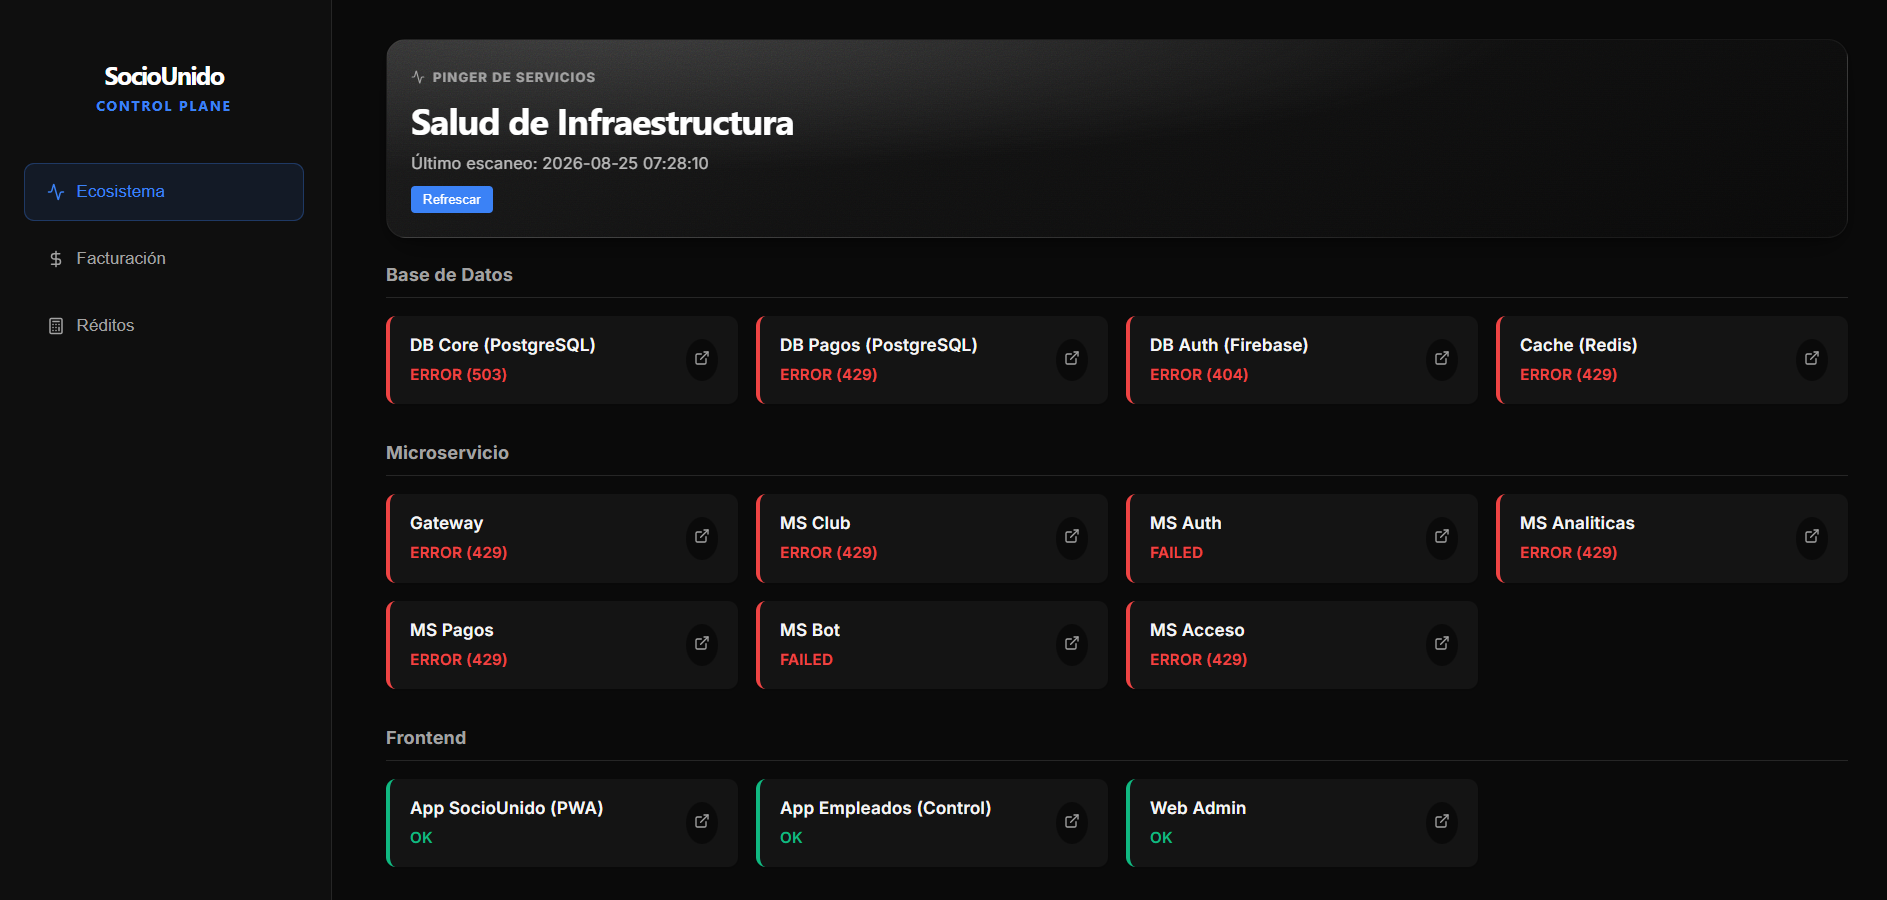
\includegraphics[width=0.85\textwidth]{img/healthchecker/healthchecker1.png}}
    \caption{Estado actual de las instancias y servicios desplegados.}
    \label{fig:ui_healthchecker1}
\end{figure}

\begin{figure}[h!]
    \centering
    \fbox{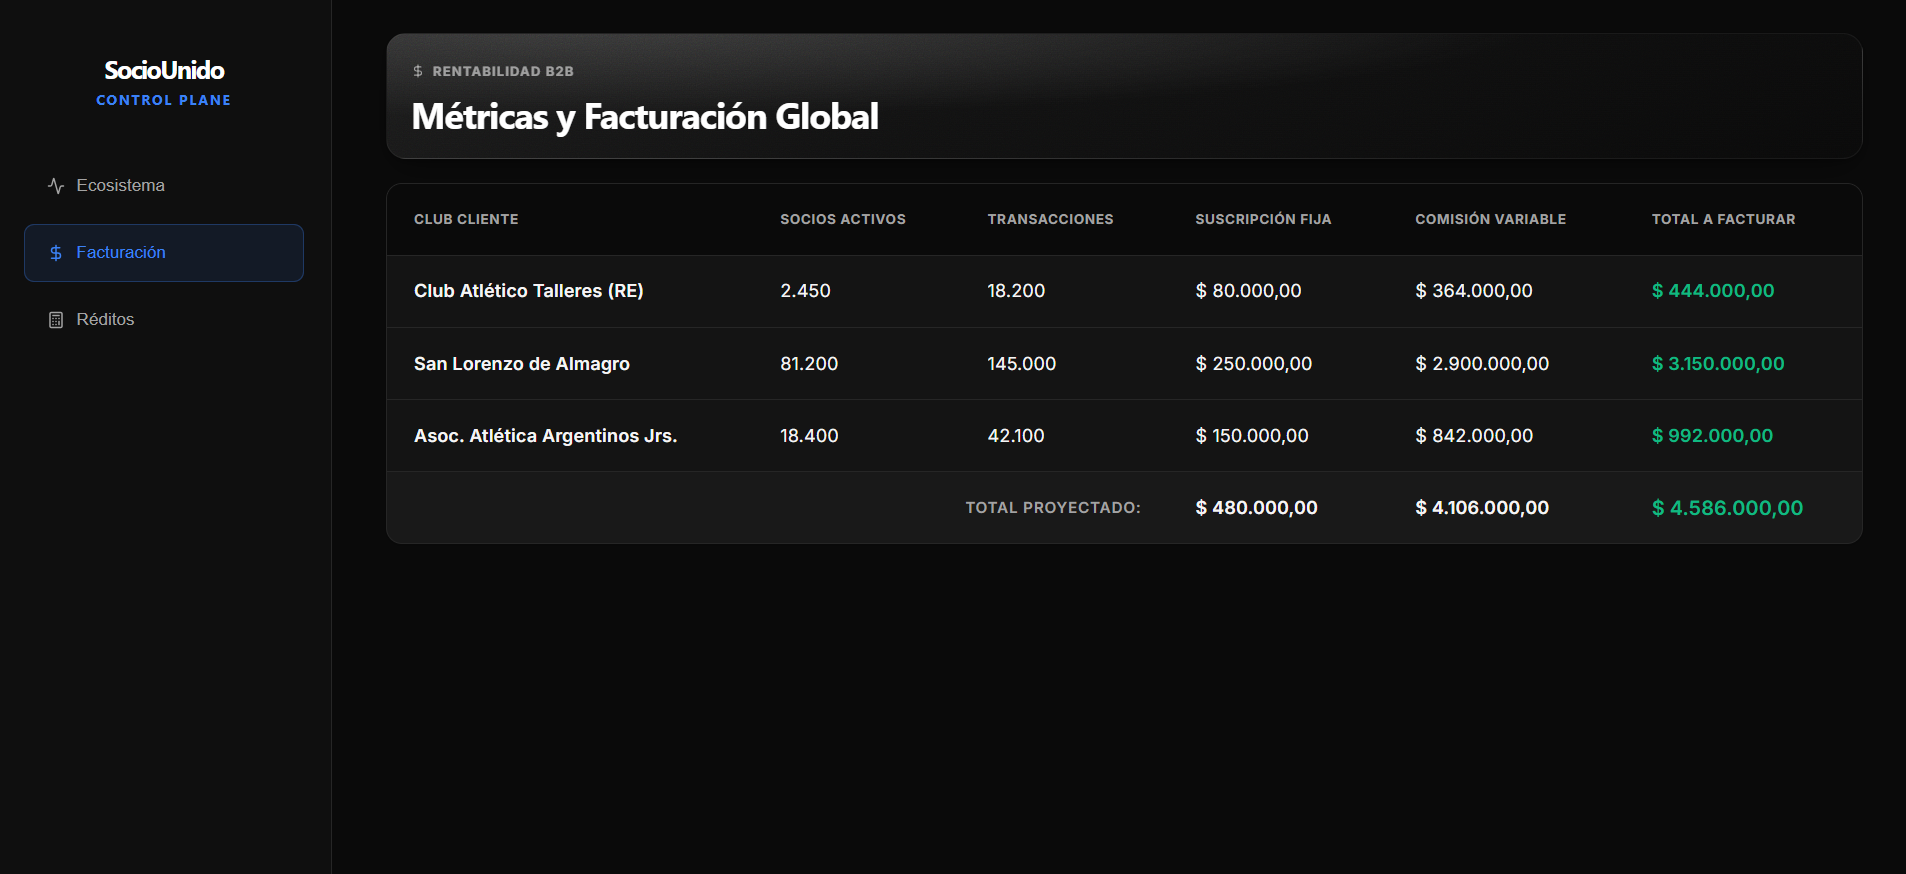
\includegraphics[width=0.85\textwidth]{img/healthchecker/healthchecker2.png}}
    \caption{Métricas de facturación de los clubes en el ecosistema.}
    \label{fig:ui_healthchecker2}
\end{figure}

\begin{figure}[h!]
    \centering
    \fbox{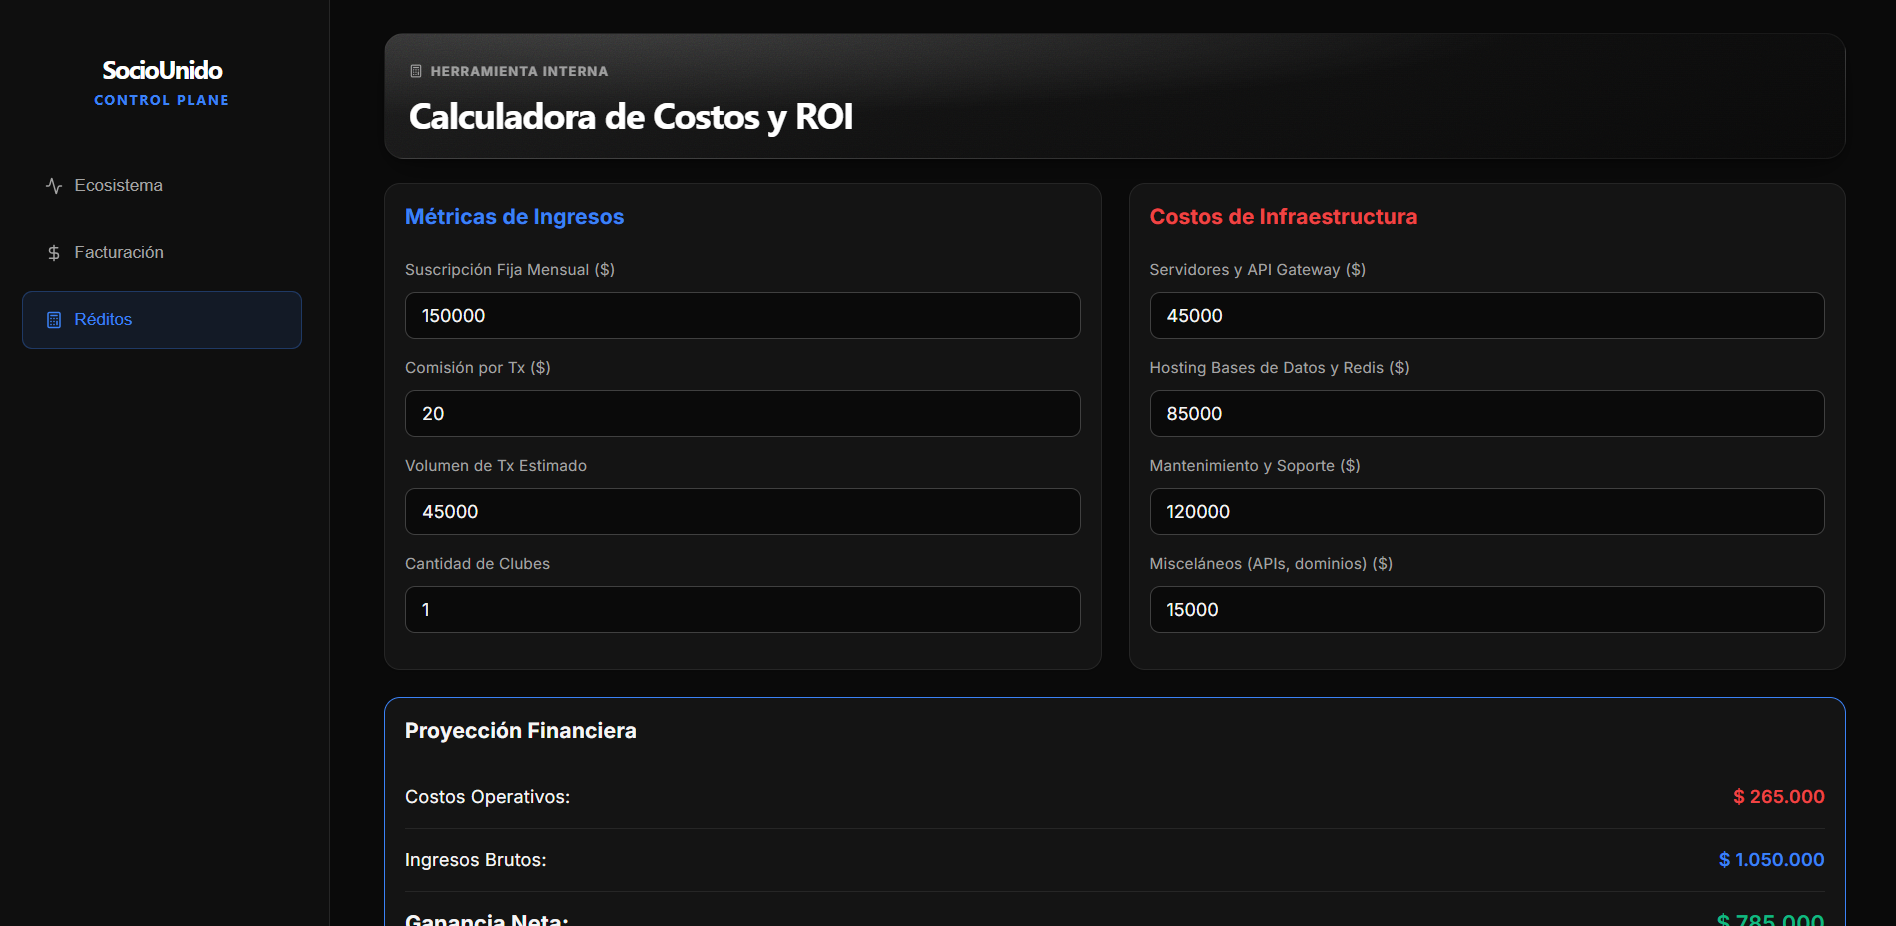
\includegraphics[width=0.85\textwidth]{img/healthchecker/healthchecker3.png}}
    \caption{Herramientas para realizar análisis comerciales y proyecciones.}
    \label{fig:ui_healthchecker3}
\end{figure}

\newpage

\subsection{Plataforma web (Panel de gestión)}

\subsubsection{Login y autenticación}
\begin{figure}[h!]
    \centering
    \textbf{Marca blanca} \\ \vspace{0.2cm}
    \fbox{
\includegraphics[width=0.9\textwidth]{img/plataforma-web/login-neutro.jpeg}} \\
    \vspace{0.8cm}
    \textbf{Mamelodi Sundowns} \\ \vspace{0.2cm}
    \fbox{
\includegraphics[width=0.9\textwidth]{img/plataforma-web/login-mamelodi.jpeg}}
    \caption{Comparativa de vistas: Login y autenticación.}
\end{figure}

\newpage

\subsubsection{Inicio (Home)}
\begin{figure}[h!]
    \centering
    \textbf{Marca blanca} \\ \vspace{0.2cm}
    \fbox{
\includegraphics[width=\textwidth]{img/plataforma-web/home-neutro.jpeg}} \\
    \vspace{0.8cm}
    \textbf{Mamelodi Sundowns} \\ \vspace{0.2cm}
    \fbox{
\includegraphics[width=\textwidth]{img/plataforma-web/home-mamelodi.jpeg}}
    \caption{Comparativa de vistas: Panel principal (Home).}
\end{figure}

\newpage

\subsubsection{Métricas y estadísticas}
\begin{figure}[h!]
    \centering
    \textbf{Marca blanca} \\ \vspace{0.2cm}
    \fbox{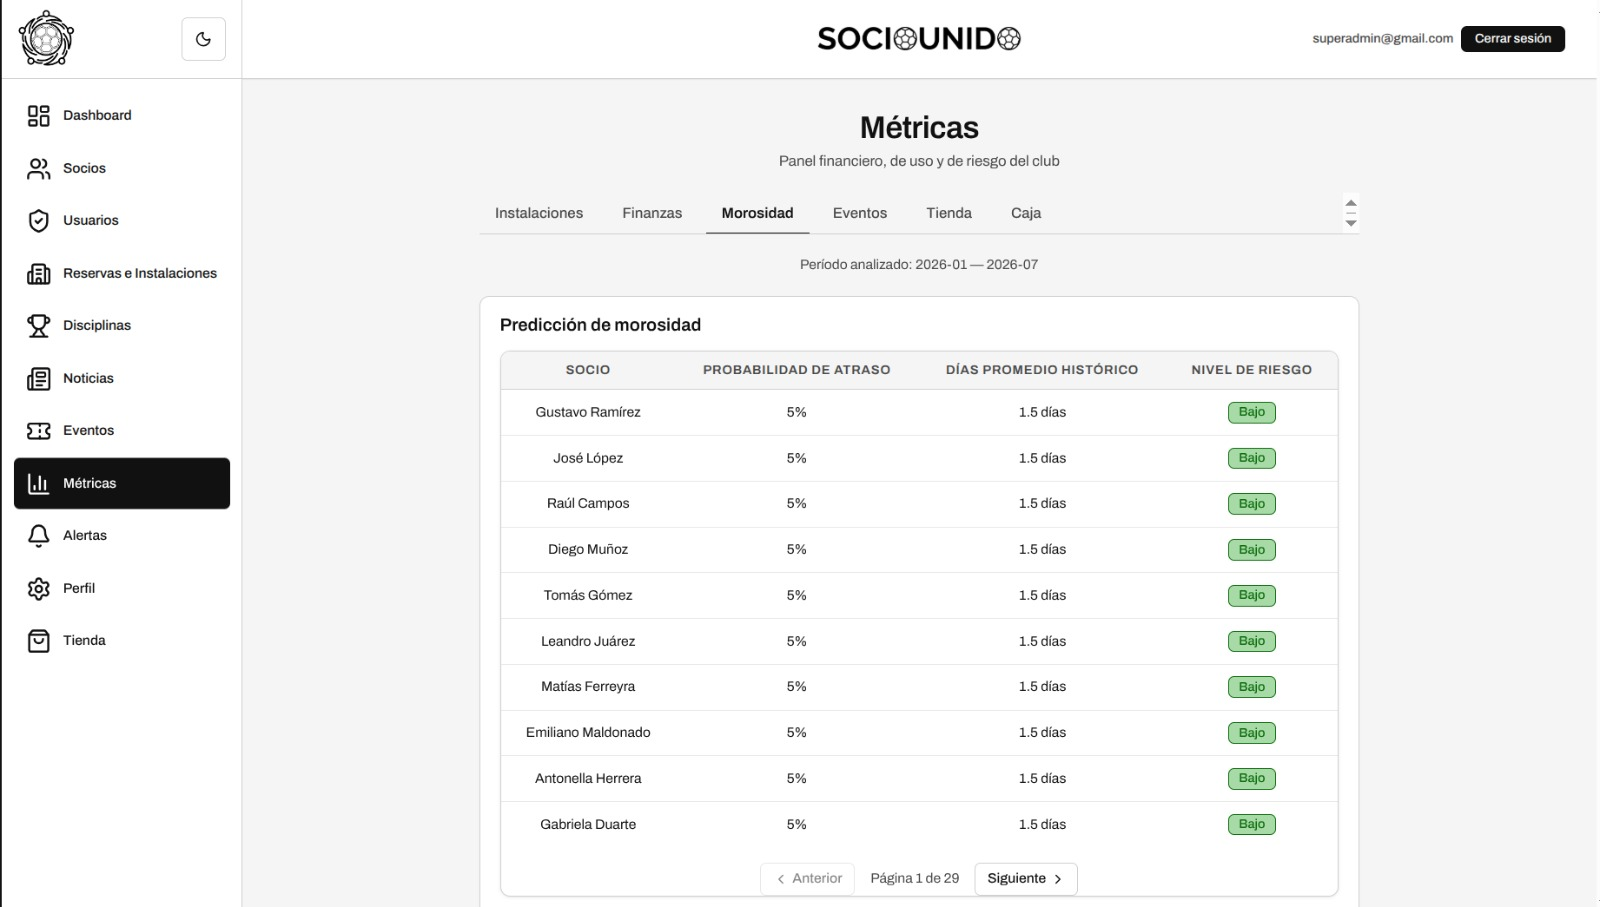
\includegraphics[width=\textwidth]{img/plataforma-web/metricas-neutro.jpeg}} \\
    \vspace{0.8cm}
    \textbf{Mamelodi Sundowns} \\ \vspace{0.2cm}
    \fbox{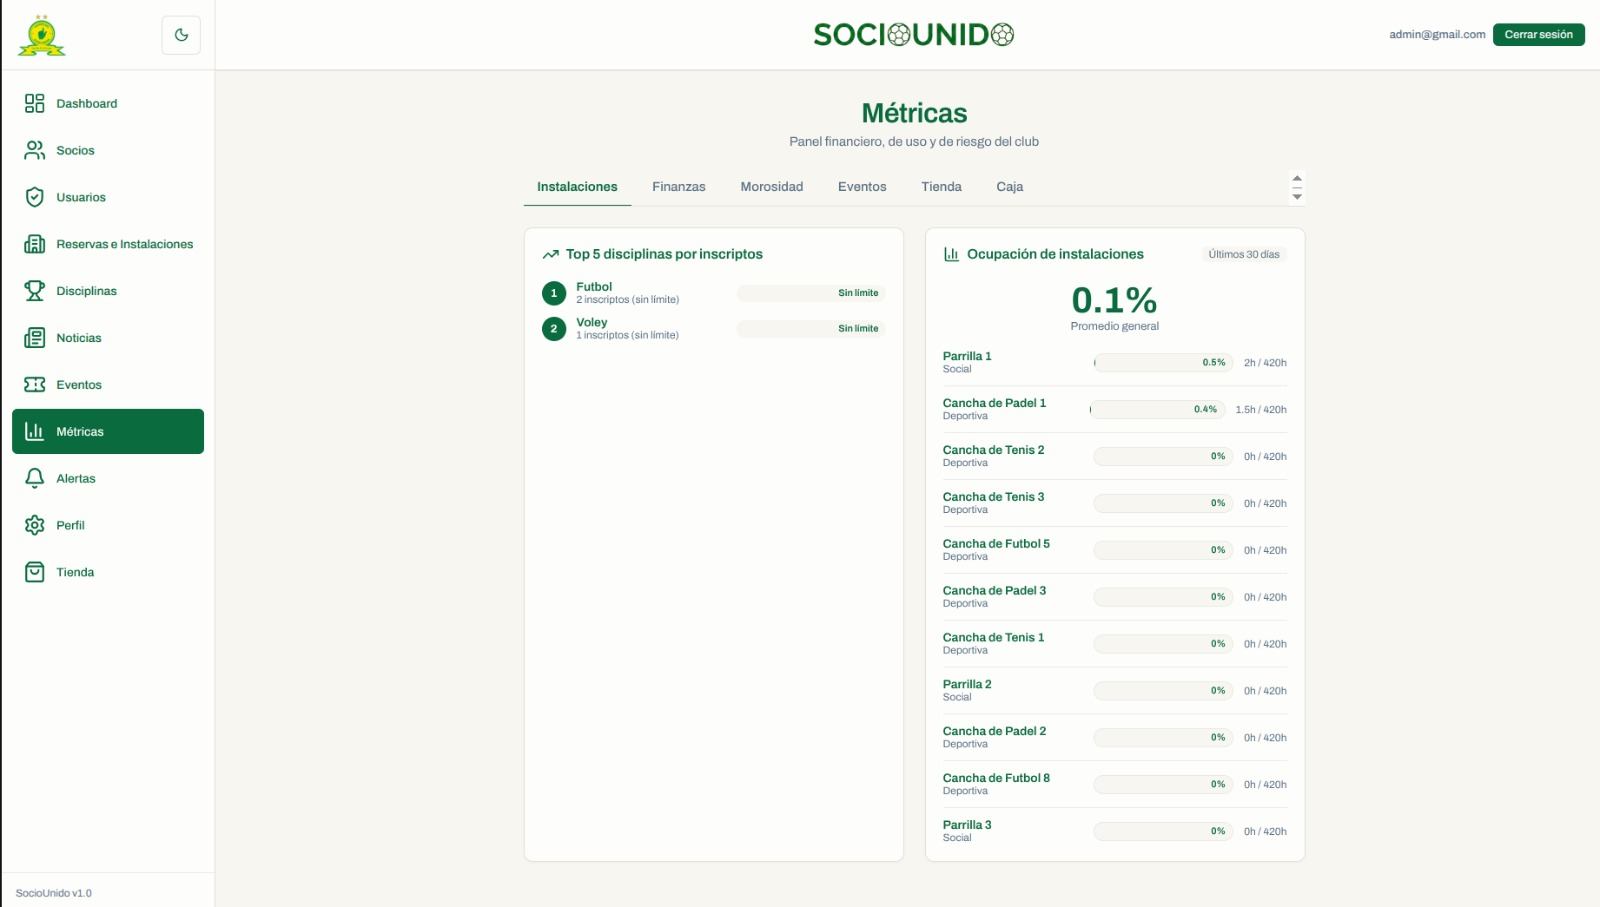
\includegraphics[width=\textwidth]{img/plataforma-web/metricas-mamelodi.jpeg}}
    \caption{Comparativa de vistas: Panel de métricas y estadísticas.}
\end{figure}

\newpage

\subsubsection{Gestión de socios y perfil específico}
\begin{figure}[h!]
    \centering
    \textbf{Padrón general (MSU)} \\ \vspace{0.2cm}
    \fbox{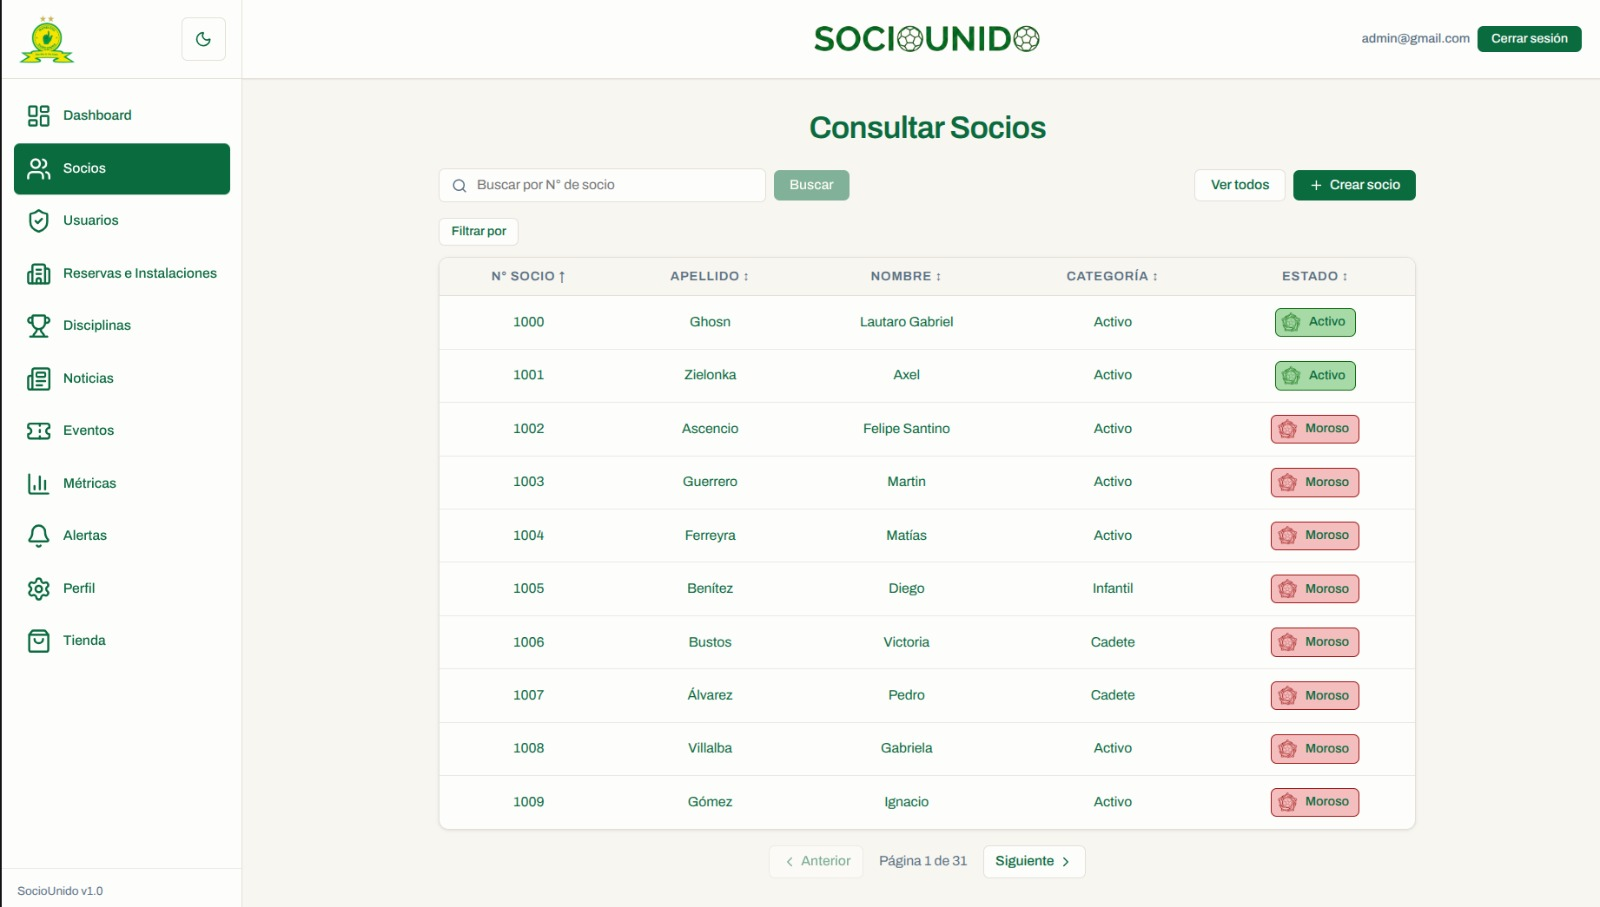
\includegraphics[width=\textwidth]{img/plataforma-web/socios-mamelodi.jpeg}} \\
    \vspace{0.8cm}
    \textbf{Perfil de socio (MSU)} \\ \vspace{0.2cm}
    \fbox{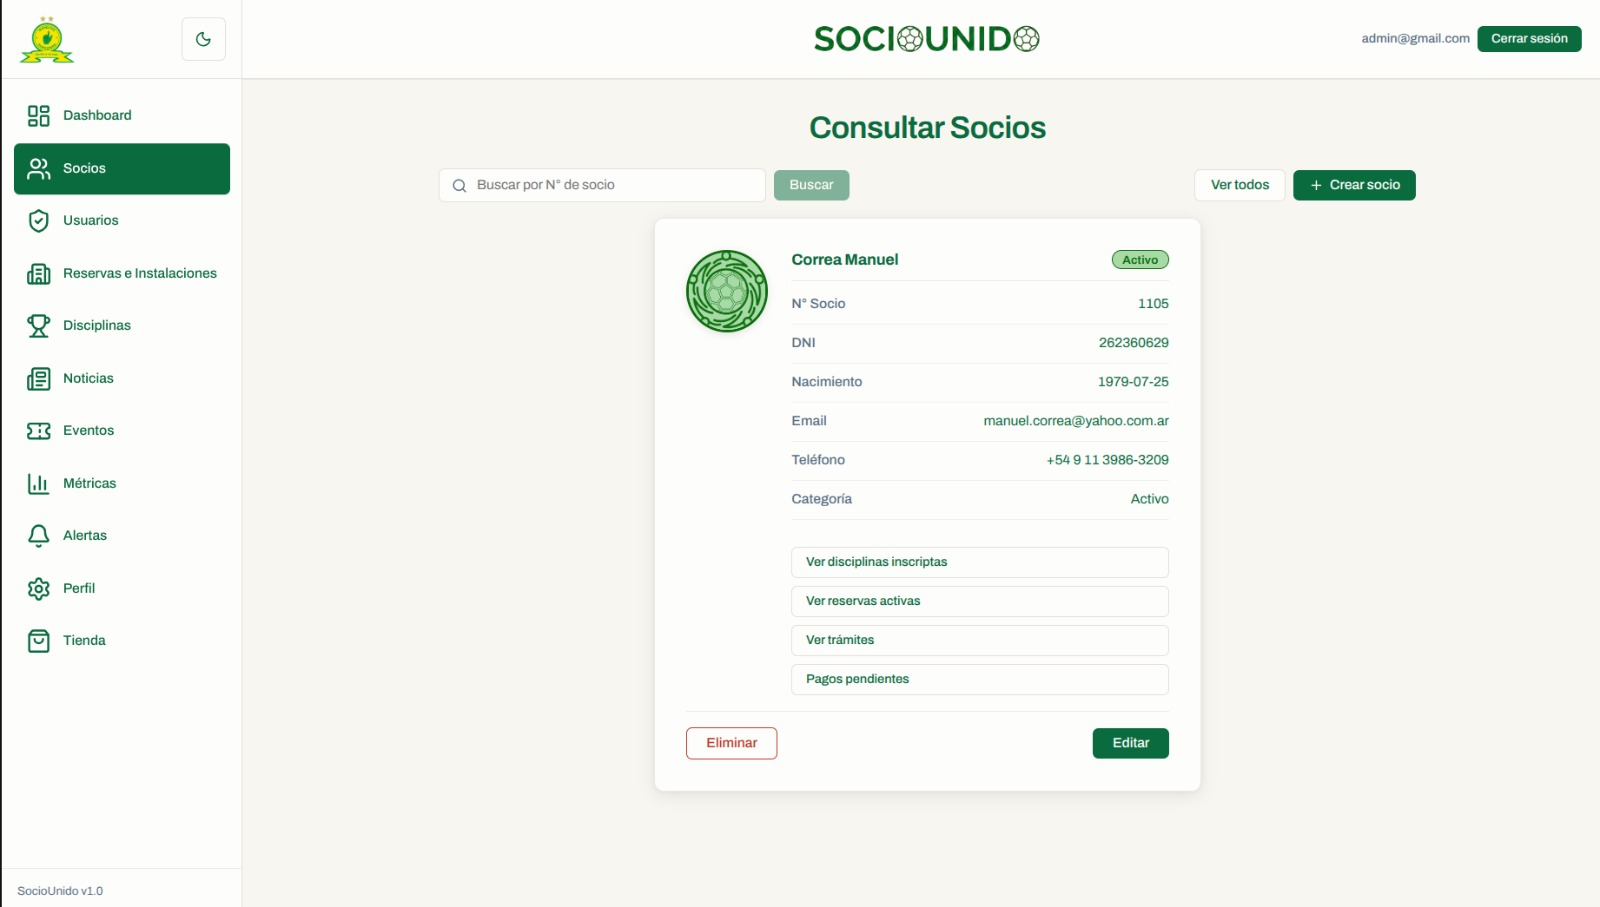
\includegraphics[width=\textwidth]{img/plataforma-web/socio-especifico-mamelodi.jpeg}}
    \caption{Vistas de gestión societaria implementadas para el club de ejemplo.}
\end{figure}

\newpage

\subsubsection{Gestión de disciplinas y tienda}
\begin{figure}[h!]
    \centering
    \textbf{Disciplinas general (MSU)} \\ \vspace{0.2cm}
    \fbox{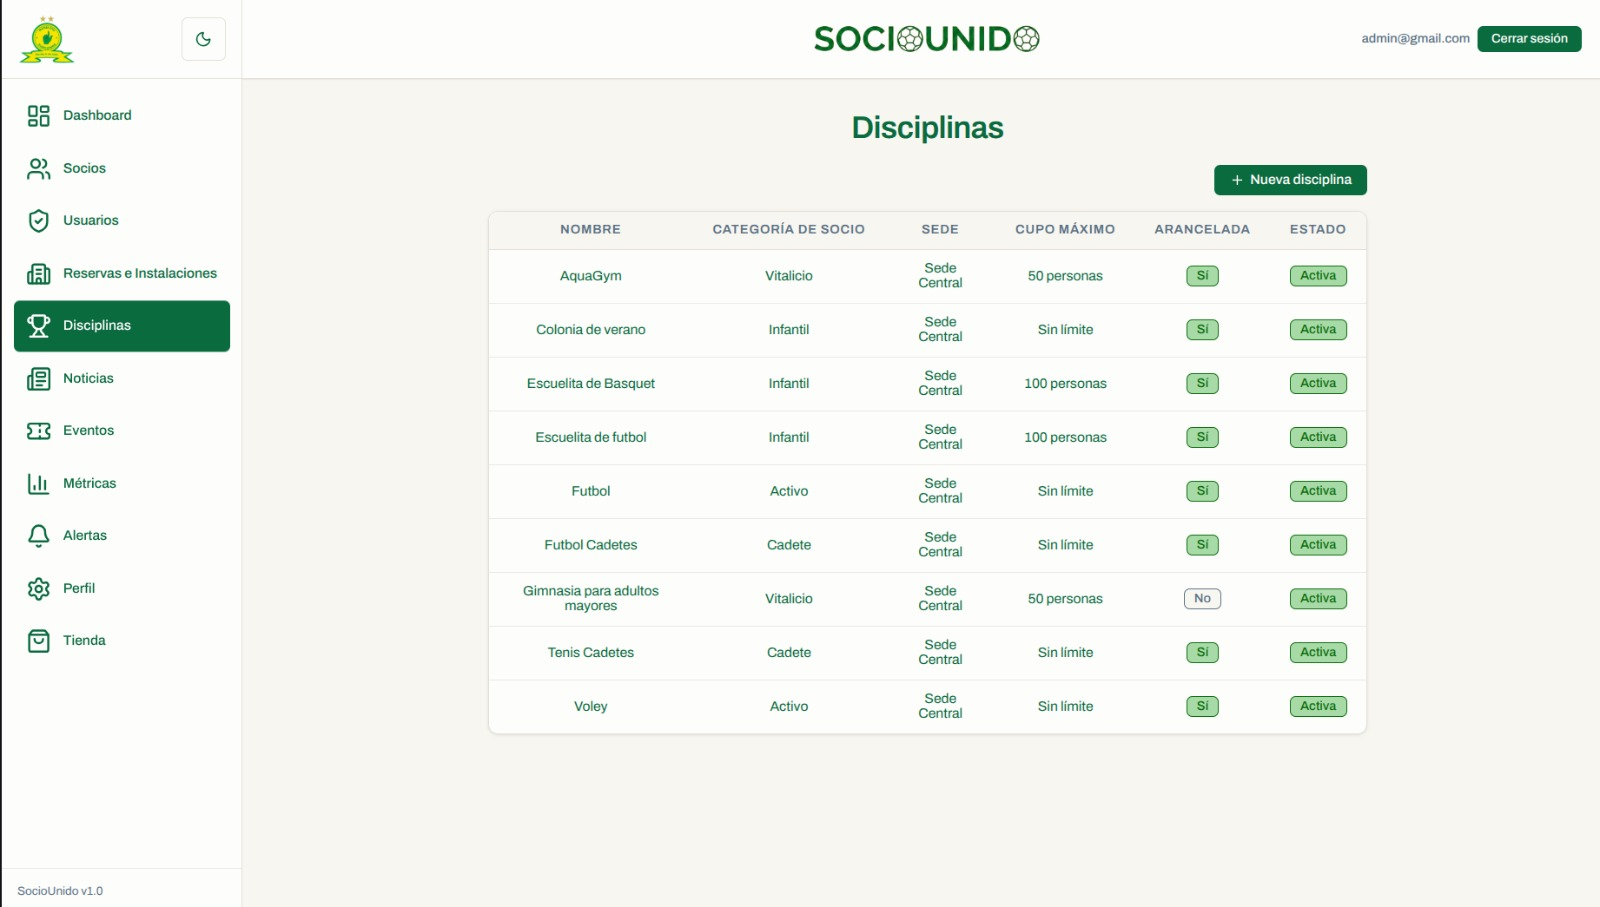
\includegraphics[width=\textwidth]{img/plataforma-web/disciplinas-mamelodi.jpeg}} \\
    \vspace{0.8cm}
    \textbf{Tienda institucional (MSU)} \\ \vspace{0.2cm}
    \fbox{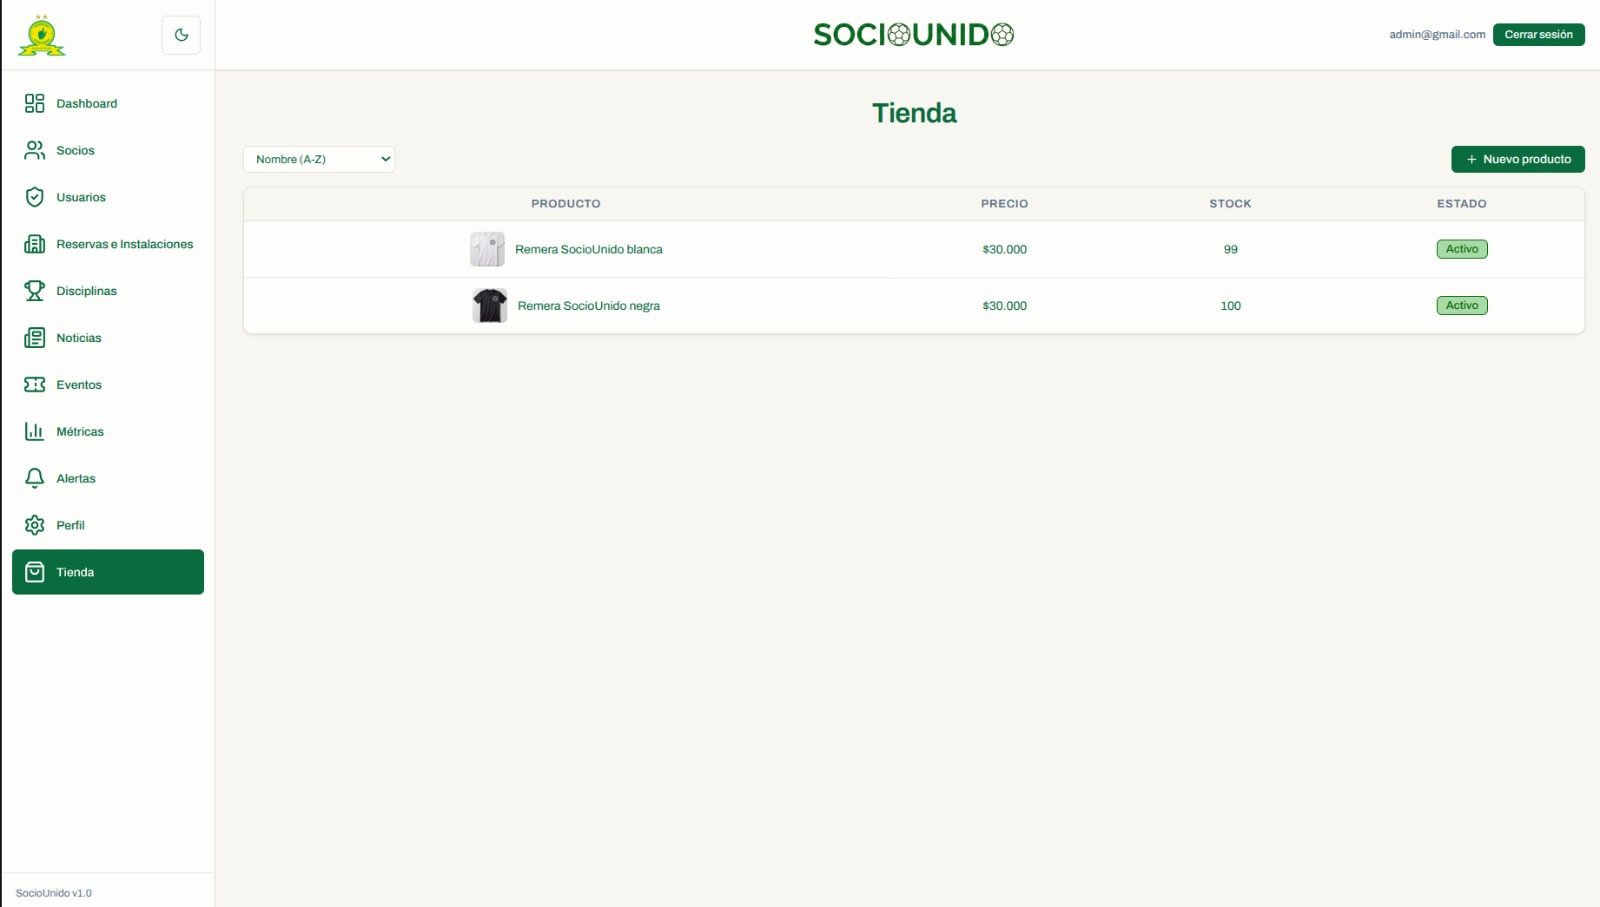
\includegraphics[width=\textwidth]{img/plataforma-web/tienda-mamelodi.jpeg}}
    \caption{Vistas de disciplinas y e-commerce implementadas para el club de ejemplo.}
\end{figure}

\newpage

\subsection{App del socio (PWA)}

% --- BLOQUE 1: LOGIN SOCIO ---
\begin{figure}[h!]
    \centering
    \begin{minipage}{0.28\textwidth}
        \centering
        \textbf{Marca blanca} \\ \vspace{0.2cm}
        \fbox{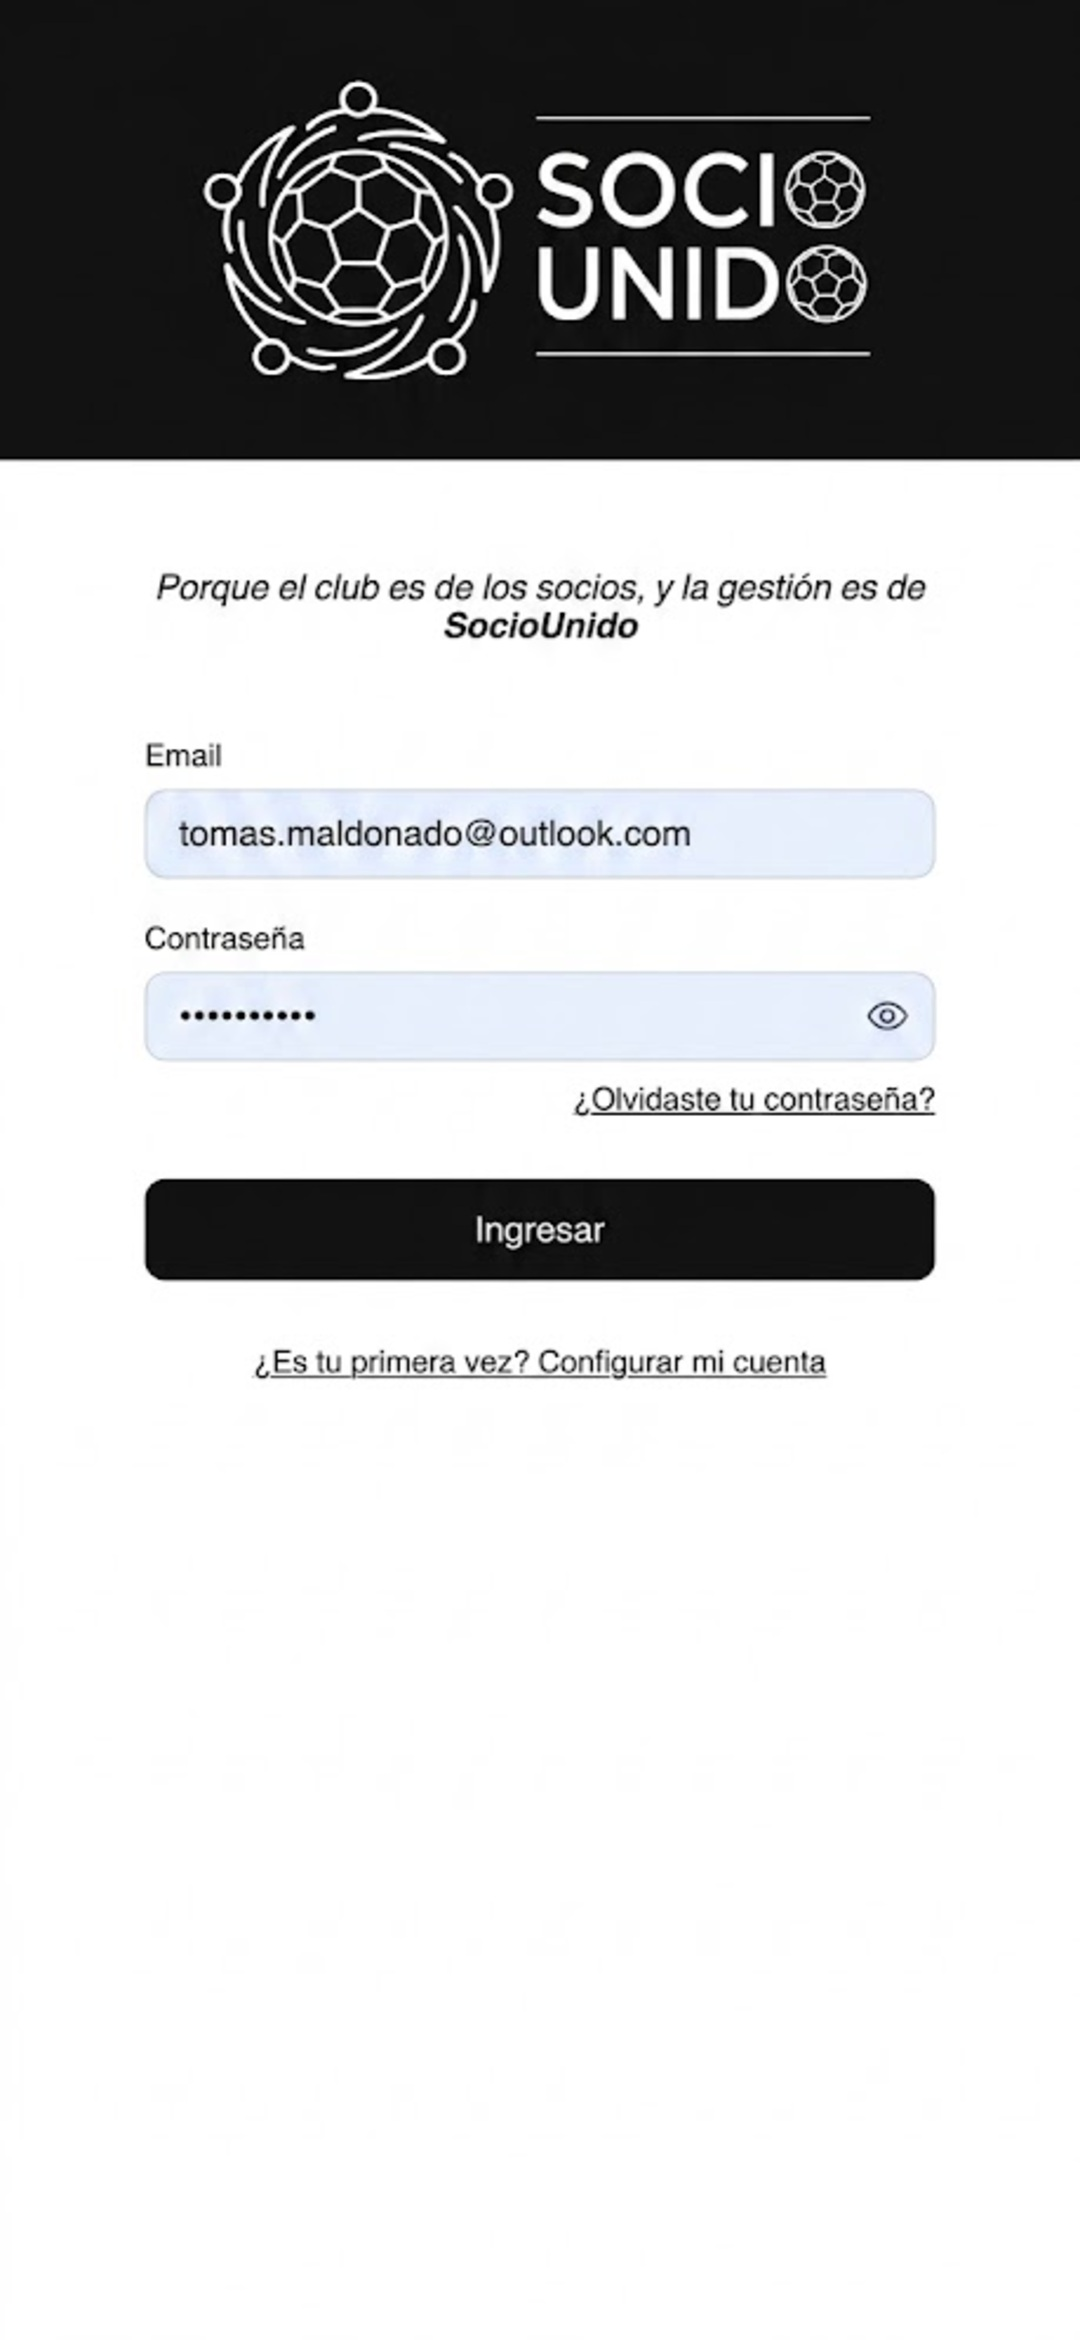
\includegraphics[width=\textwidth]{img/app-socio/login-neutro.jpg}}
    \end{minipage}\hspace{0.5cm}
    \begin{minipage}{0.28\textwidth}
        \centering
        \textbf{Mamelodi Sundowns} \\ \vspace{0.2cm}
        \fbox{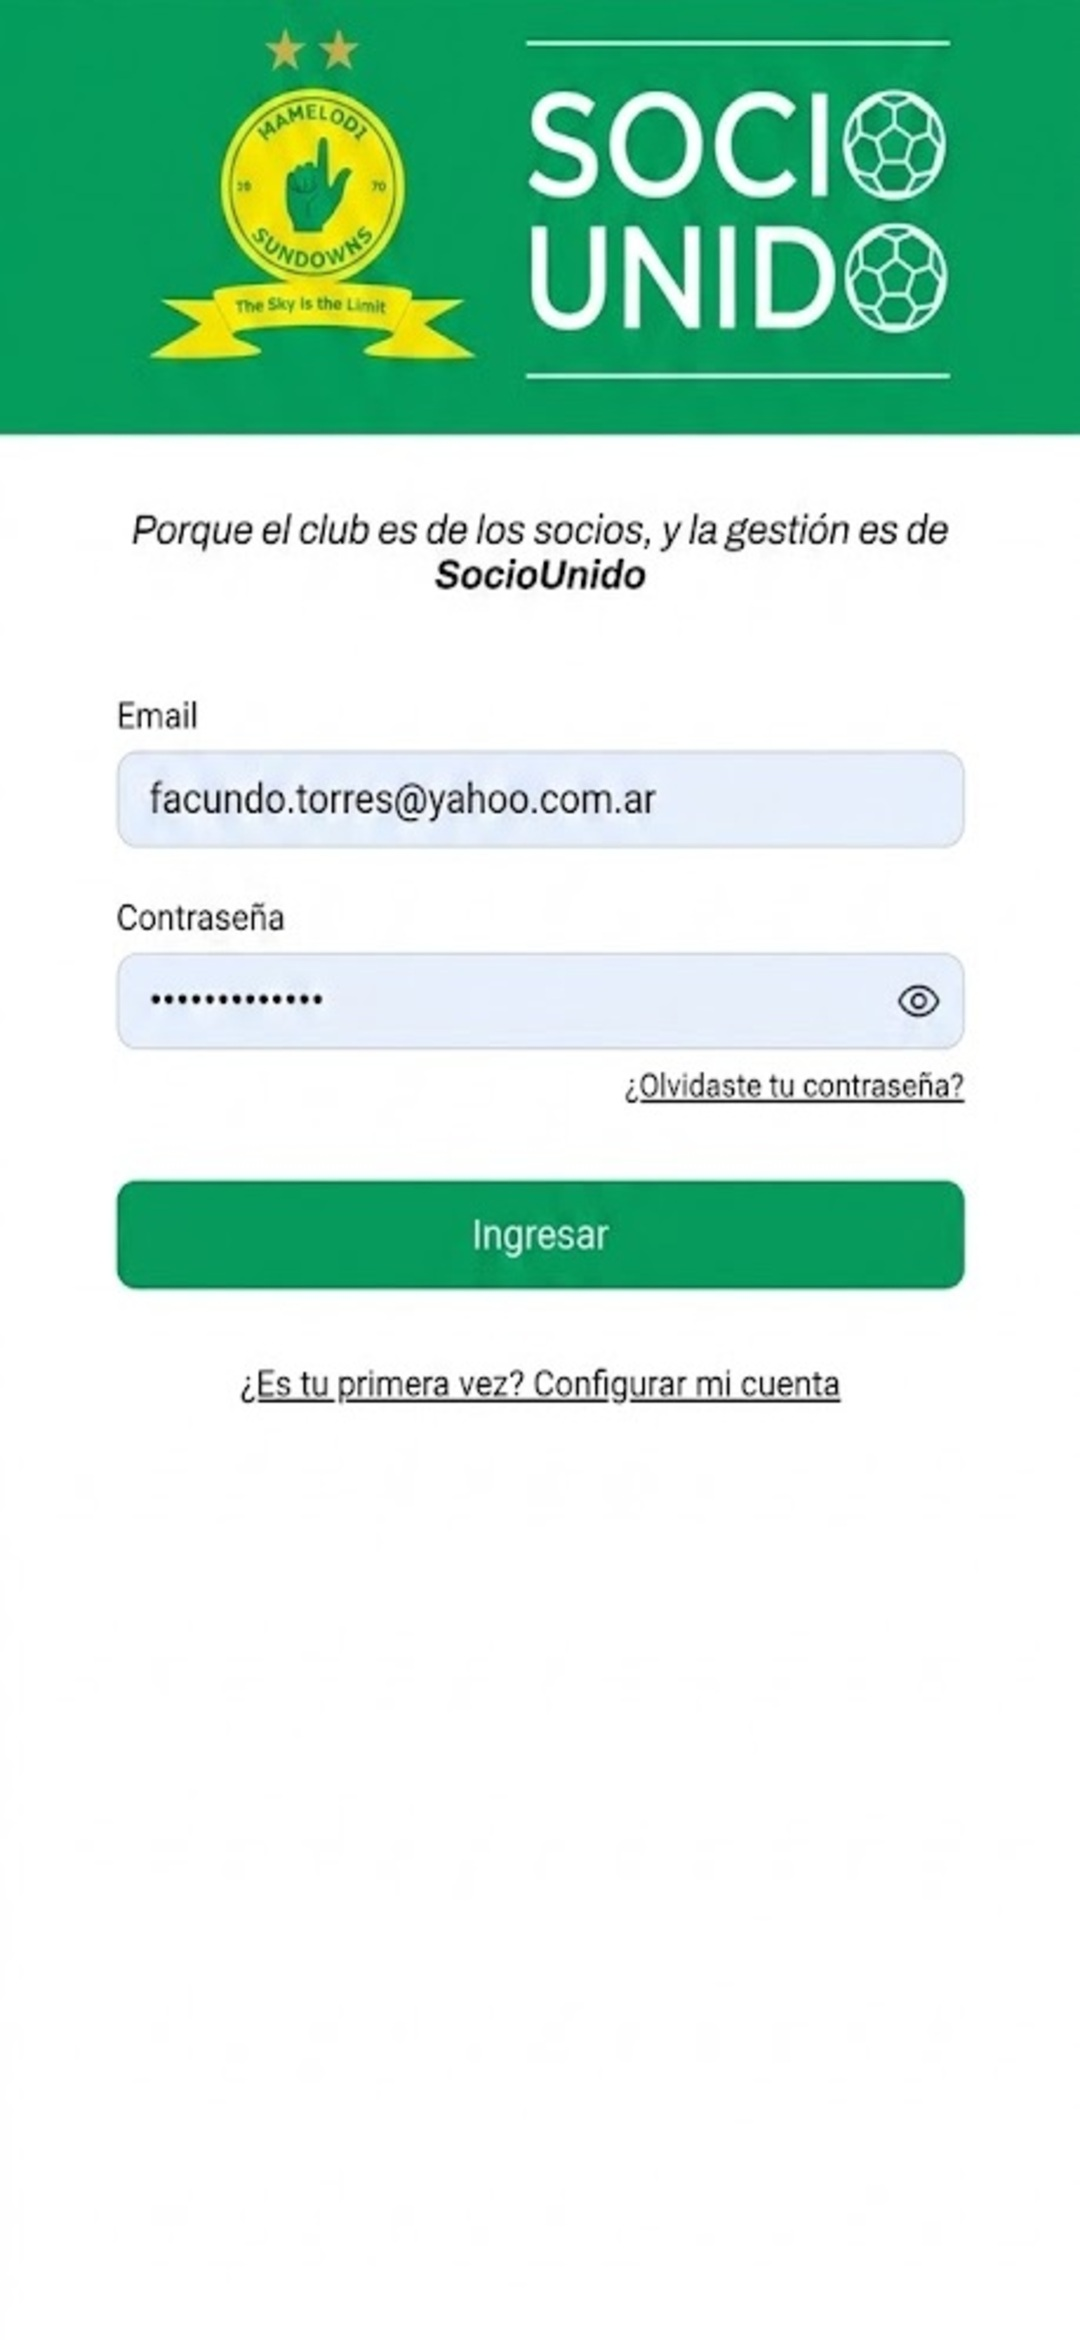
\includegraphics[width=\textwidth]{img/app-socio/login-mamelodi.jpg}}
    \end{minipage}
    \caption{Pantallas de acceso (Login) de la App del Socio.}
    \label{fig:socio_login}
\end{figure}

% --- BLOQUE 2: DASHBOARD SOCIO ---
\begin{figure}[h!]
    \centering
    \begin{minipage}{0.28\textwidth}
        \centering
        \textbf{Marca blanca} \\ \vspace{0.2cm}
        \fbox{
\includegraphics[width=\textwidth]{img/app-socio/home-neutro.jpg}}
    \end{minipage}\hspace{0.5cm}
    \begin{minipage}{0.28\textwidth}
        \centering
        \textbf{Mamelodi Sundowns} \\ \vspace{0.2cm}
        \fbox{
\includegraphics[width=\textwidth]{img/app-socio/home-mamelodi.jpg}}
    \end{minipage}
    \caption{Inicio (Dashboard del socio).}
    \label{fig:socio_home}
\end{figure}

\newpage

% --- BLOQUE 3: PERFIL Y PAGOS SOCIO ---
\begin{figure}[h!]
    \centering
    \begin{minipage}{0.3\textwidth}
        \centering
        \textbf{Perfil (MSU)} \\ \vspace{0.2cm}
        \fbox{
\includegraphics[width=\textwidth]{img/app-socio/perfil-mamelodi.jpg}}
    \end{minipage}\hspace{0.5cm}
    \begin{minipage}{0.3\textwidth}
        \centering
        \textbf{Pagos (MSU)} \\ \vspace{0.2cm}
        \fbox{
\includegraphics[width=\textwidth]{img/app-socio/pagos-mamelodi.jpg}}
    \end{minipage}
    \caption{Perfil de usuario y gestión de pagos.}
    \label{fig:socio_pagos}
\end{figure}

% --- BLOQUE 4: CARNET DIGITAL SOCIO ---
\begin{figure}[h!]
    \centering
    \begin{minipage}{0.3\textwidth}
        \centering
        \textbf{Marca blanca} \\ \vspace{0.2cm}
        \fbox{
\includegraphics[width=\textwidth]{img/app-socio/carnet-neutro.jpg}}
    \end{minipage}\hspace{0.5cm}
    \begin{minipage}{0.3\textwidth}
        \centering
        \textbf{Mamelodi Sundowns} \\ \vspace{0.2cm}
        \fbox{
\includegraphics[width=\textwidth]{img/app-socio/carnet-mamelodi.jpg}}
    \end{minipage}
    \caption{Carnet digital y acceso inteligente.}
    \label{fig:socio_carnet}
\end{figure}

\newpage

\subsection{App de empleados (PWA)}

% --- BLOQUE 5: LOGIN Y HOME TRABAJADORES ---
\begin{figure}[h!]
    \centering
    \begin{minipage}{0.28\textwidth}
        \centering
        \textbf{Acceso (MSU)} \\ \vspace{0.2cm}
        \fbox{
\includegraphics[width=\textwidth]{img/app-trabajadores/login-mamelodi.jpg}}
    \end{minipage}\hspace{0.5cm}
    \begin{minipage}{0.28\textwidth}
        \centering
        \textbf{Inicio (MSU)} \\ \vspace{0.2cm}
        \fbox{
\includegraphics[width=\textwidth]{img/app-trabajadores/home-mamelodi.jpg}}
    \end{minipage}
    \caption{Pantallas de acceso y menú principal de la App para Empleados.}
    \label{fig:trabajadores_inicio}
\end{figure}

% --- BLOQUE 6: ESCANEO QR TRABAJADORES ---
\begin{figure}[h!]
    \centering
    \begin{minipage}{0.28\textwidth}
        \centering
        \textbf{Marca blanca} \\ \vspace{0.2cm}
        \fbox{
\includegraphics[width=\textwidth]{img/app-trabajadores/qr-neutro.jpg}}
    \end{minipage}\hspace{0.5cm}
    \begin{minipage}{0.28\textwidth}
        \centering
        \textbf{Mamelodi Sundowns} \\ \vspace{0.2cm}
        \fbox{
\includegraphics[width=\textwidth]{img/app-trabajadores/qr-mamelodi.jpg}}
    \end{minipage}
    \caption{Módulo de escaneo de QR para control de accesos y validación de carnets.}
    \label{fig:trabajadores_qr}
\end{figure}

\newpage

\subsection{Bot conversacional (BotIn)}

\begin{figure}[h!]
    \centering
    \begin{minipage}{0.45\textwidth}
        \centering
        \textbf{Perfil institucional} \\ \vspace{0.2cm}
        \fbox{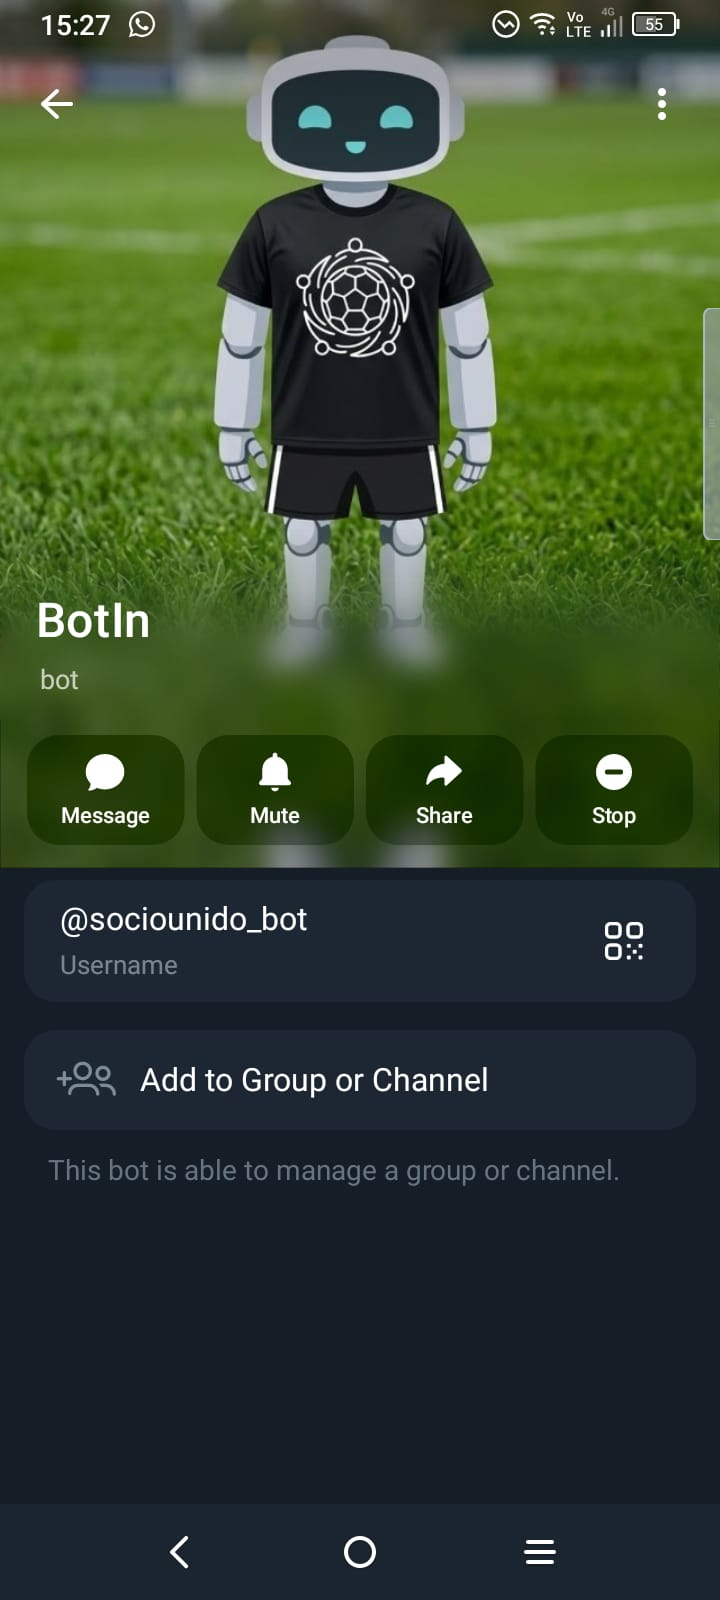
\includegraphics[width=\textwidth]{img/bot/perfil.jpeg}}
    \end{minipage}\hspace{0.5cm}
    \begin{minipage}{0.45\textwidth}
        \centering
        \textbf{Interacción (Chat)} \\ \vspace{0.2cm}
        \fbox{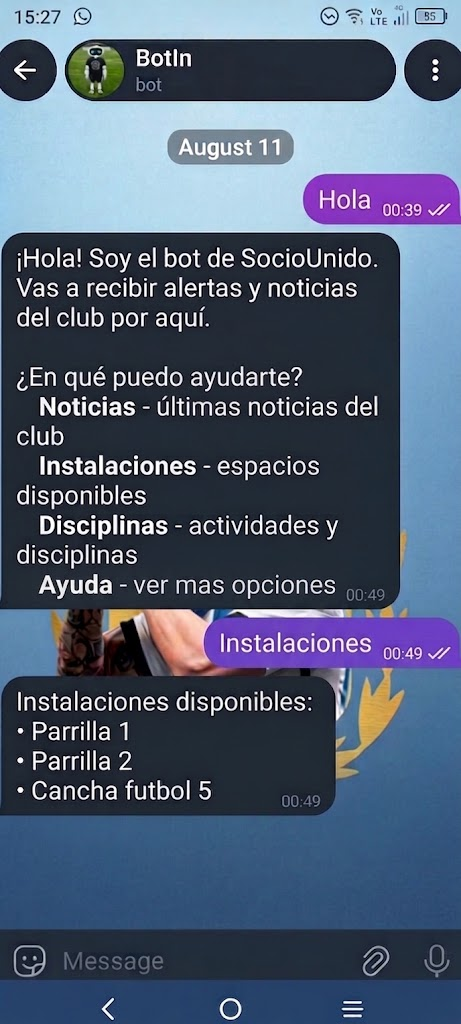
\includegraphics[width=\textwidth]{img/bot/chat.jpg}}
    \end{minipage}
    \caption{Vistas del perfil verificado y ejemplo de flujo de mensajes automatizados vía Telegram.}
    \label{fig:bot_conversacional}
\end{figure}

\newpage

\subsection{Arquitectura técnica del sistema y modelo C4}

La arquitectura de SocioUnido se rige por un paradigma orientado a microservicios desacoplados, adoptando el principio de responsabilidad única en cada componente y la segregación de persistencia de datos. Este diseño arquitectónico garantiza la escalabilidad horizontal, la tolerancia a fallos parciales y la flexibilidad para inyectar actualizaciones de código sin interrumpir el funcionamiento global del ecosistema.

\subsubsection{Estructura general de componentes y su interrelación (niveles C1 y C2)}

La visualización de la plataforma se modela mediante el estándar del modelo C4, permitiendo mapear los componentes del sistema con niveles incrementales de abstracción:

\begin{enumerate}
    \item \textbf{Nivel 1 (Contexto)}: Representa la interacción de SocioUnido con los actores humanos del sistema (socio, dirigencia y personal de control perimetral) y las entidades o plataformas externas (la pasarela transaccional de Mercado Pago, la plataforma de mensajería Telegram y los servicios auxiliares de envío de correos).
    \item \textbf{Nivel 2 (Contenedores)}: Detalla la separación física de las interfaces de usuario de \textit{frontend} (aplicaciones web y móviles progresivas desarrolladas con React) respecto a la capa de \textit{backend}, la cual se compone del portal de enlace de aplicaciones o puerta de enlace de API (\textit{API gateway}) basado en KrakenD, la suite de microservicios y la base de datos transaccional en la nube.
\end{enumerate}

\subsubsection{Diagramas de nivel 1 (Contexto) y nivel 2 (Contenedores)}

\begin{figure}[h!]
    \centering
    \fbox{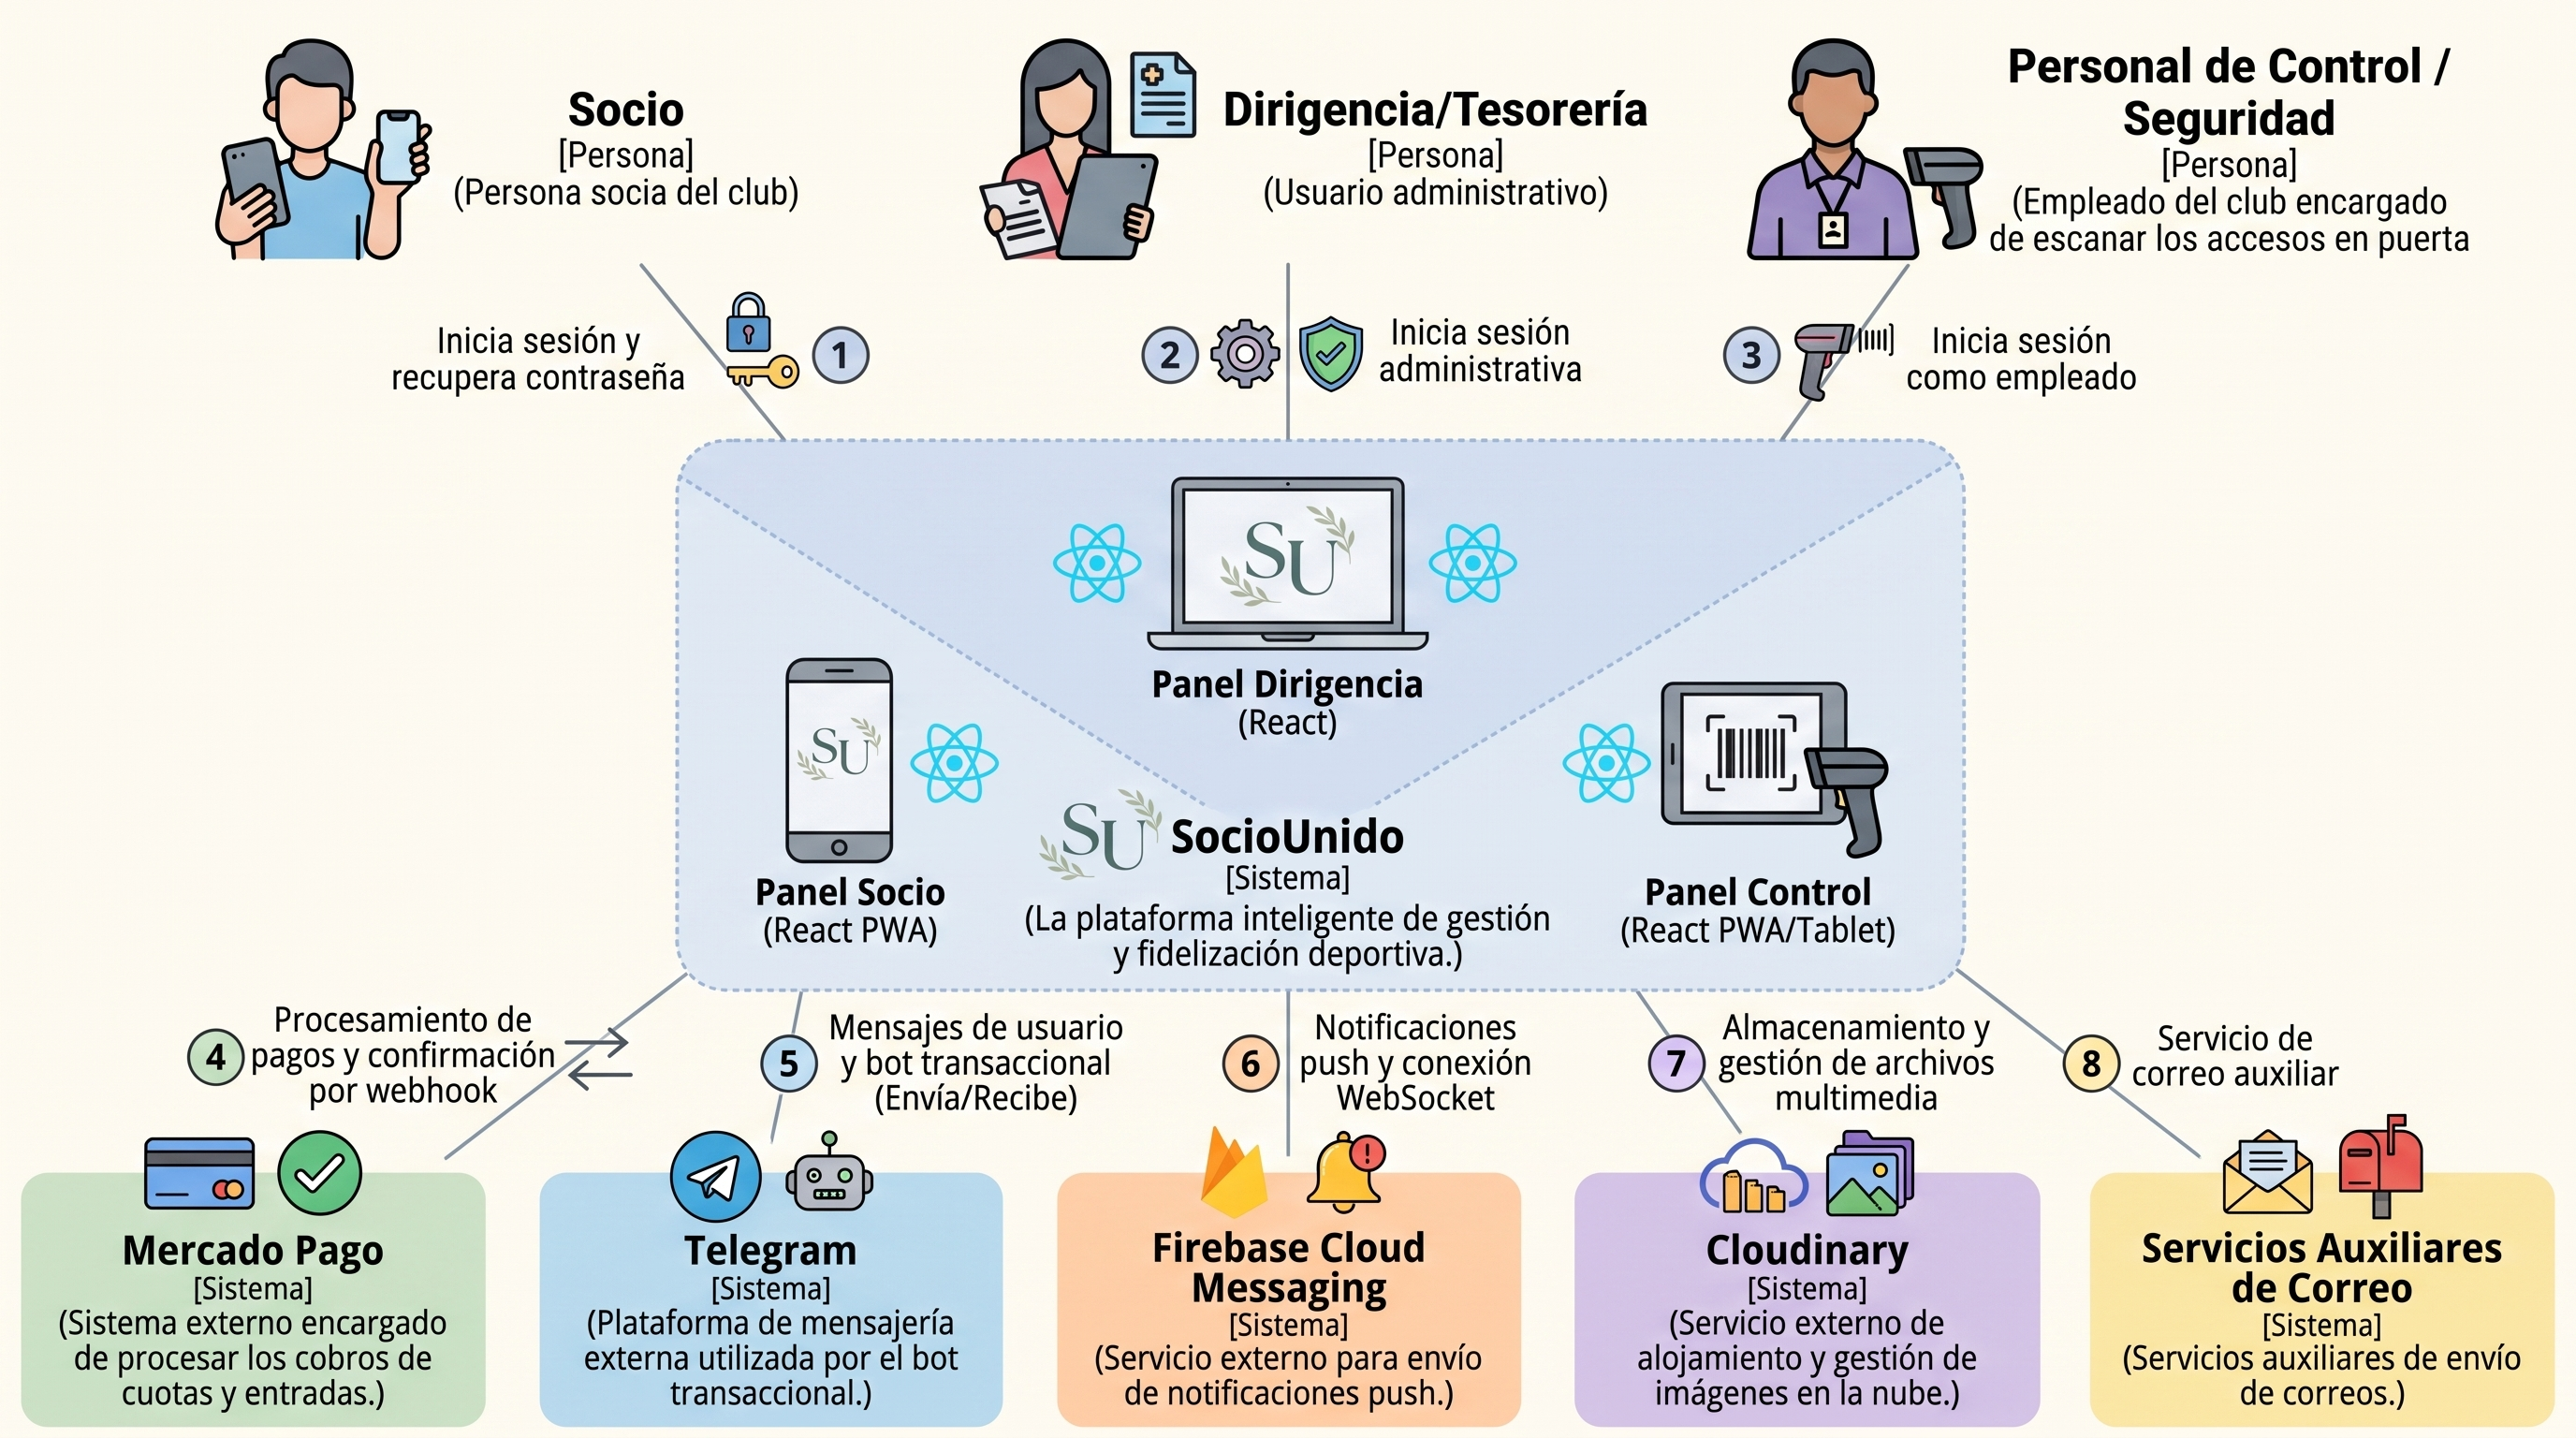
\includegraphics[width=\textwidth]{img/arquitectura/c1_contexto.jpg}}
    \caption{Diagrama de contexto (C1) simplificado del ecosistema \textit{SocioUnido} y sus fronteras de integración con actores y servicios externos.}
    \label{fig:c1_contexto}
\end{figure}

\newpage

\begin{figure}[h!]
    \centering
    \fbox{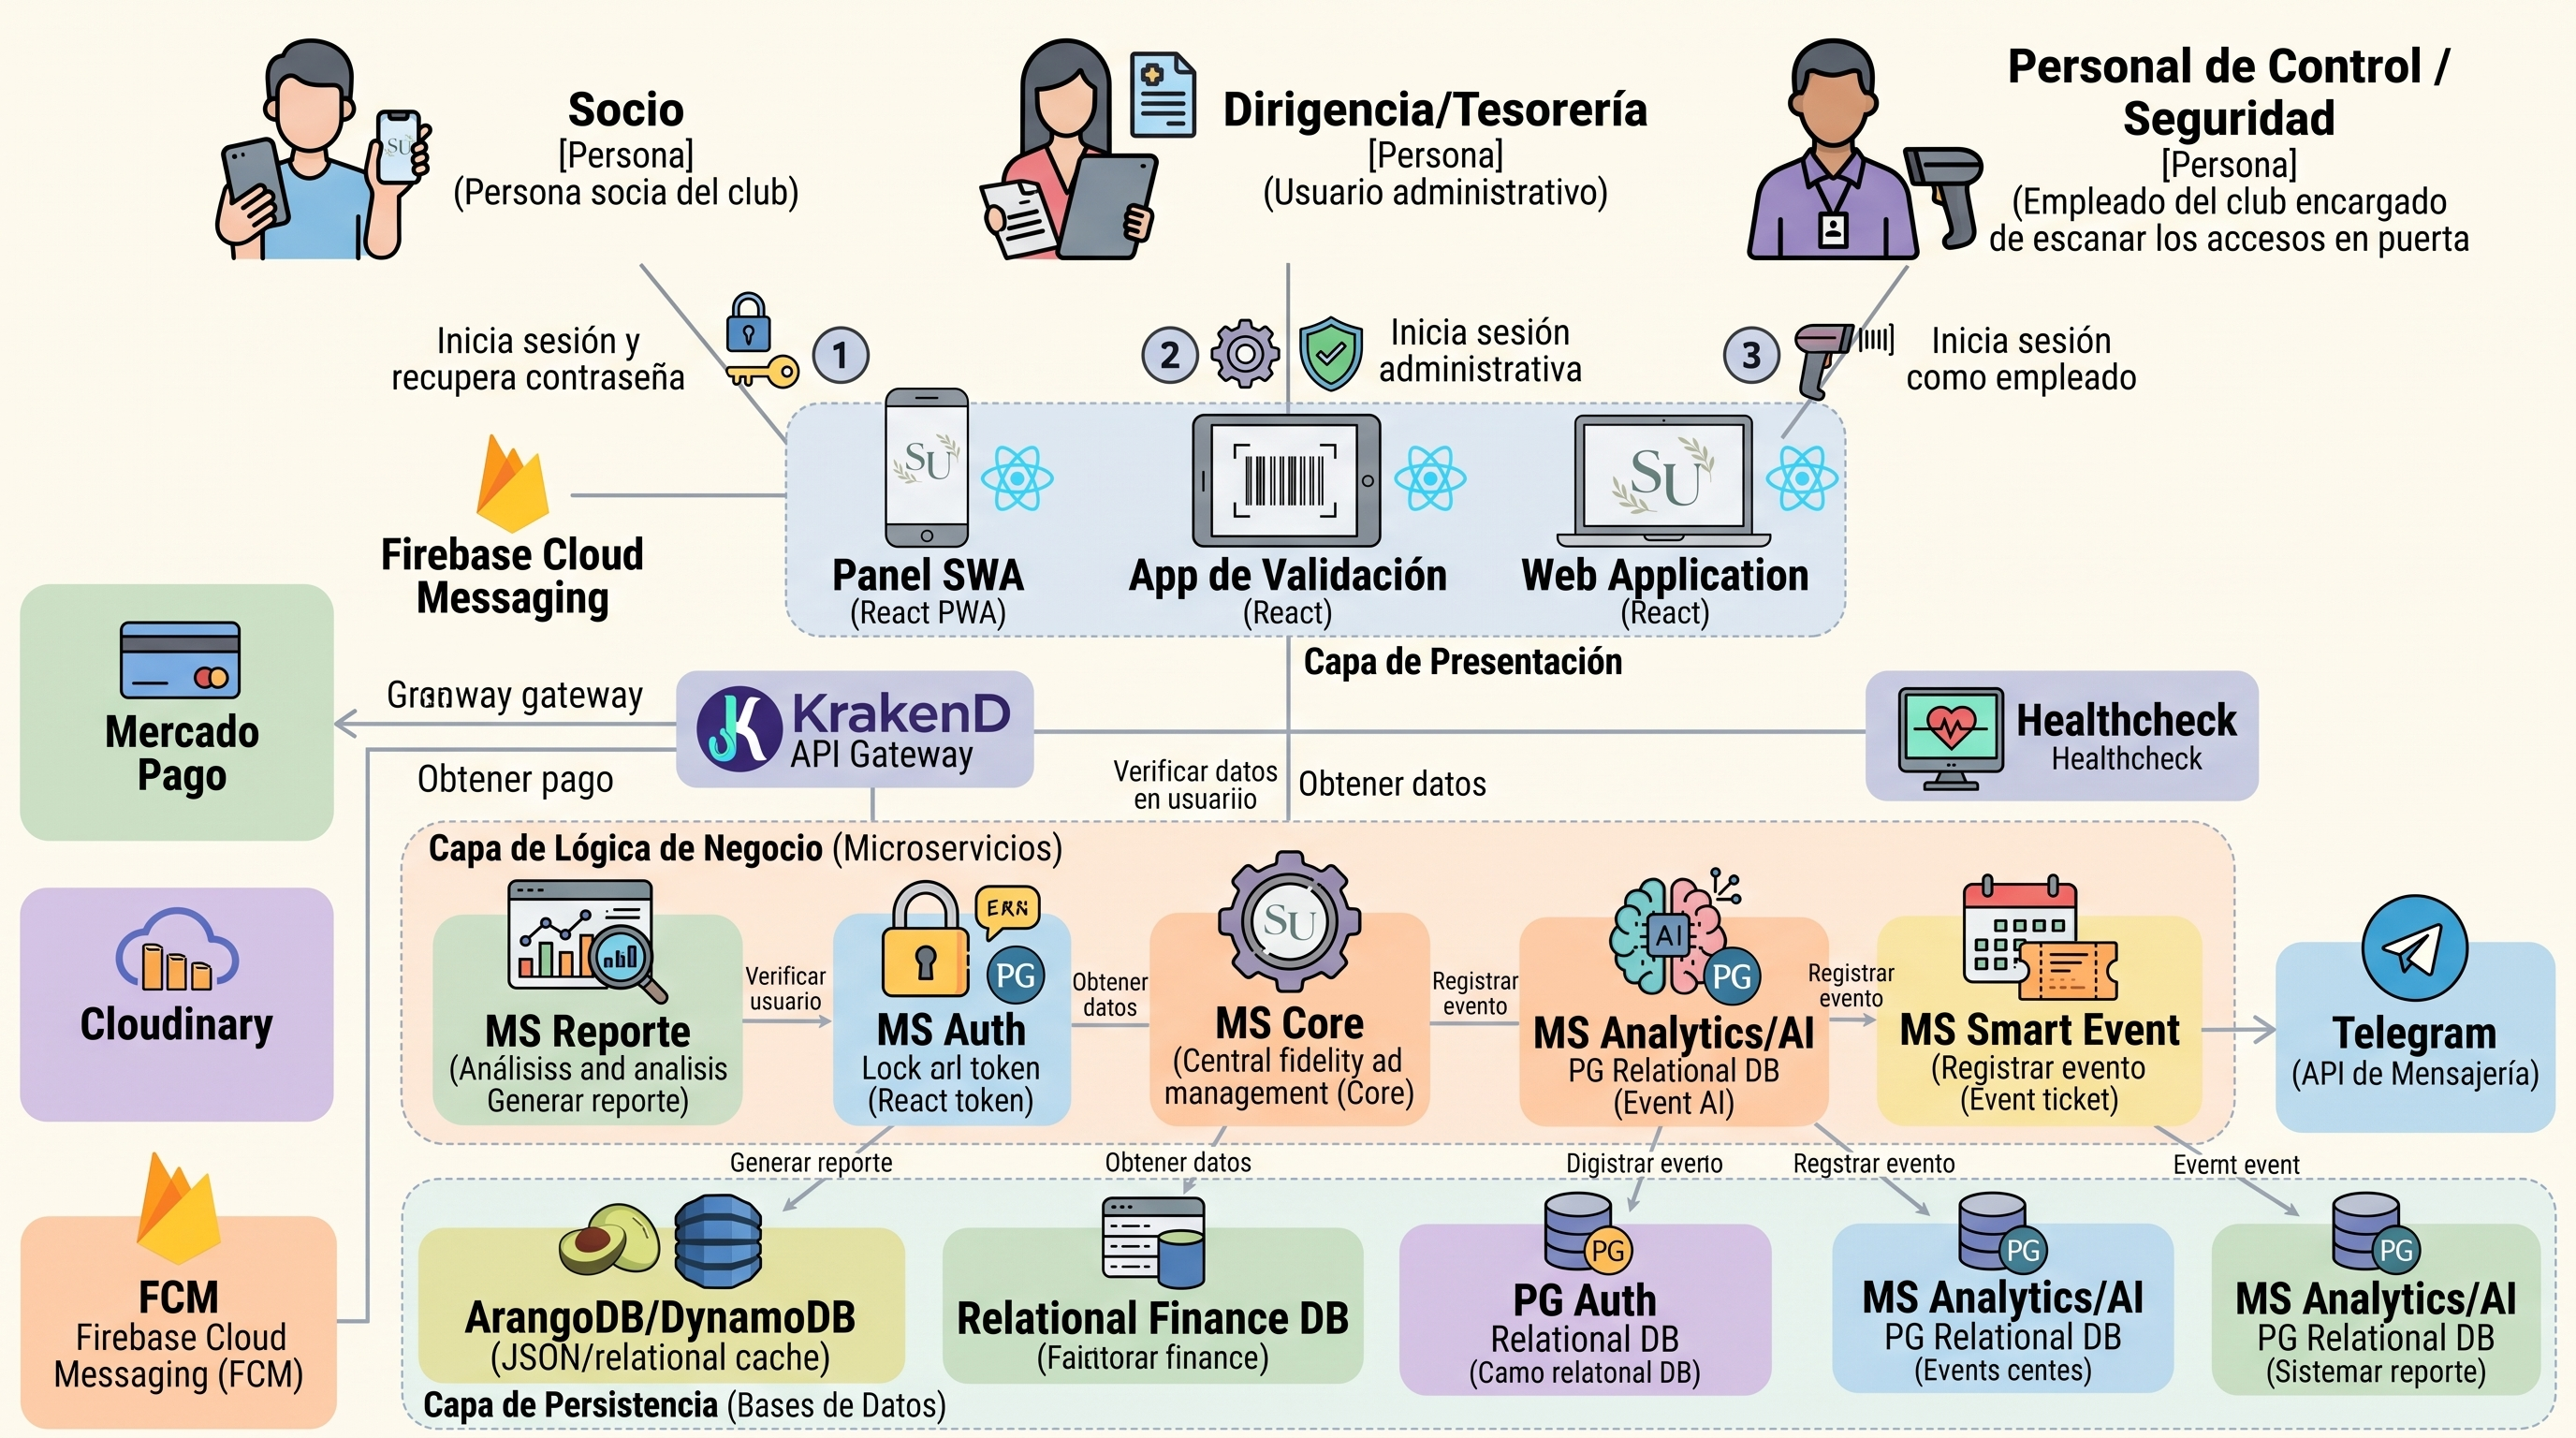
\includegraphics[width=\textwidth]{img/arquitectura/c2_componentes.jpg}}
    \caption{Diagrama de contenedores (C2) que detalla el aislamiento de las interfaces de \textit{frontend} respecto a los microservicios y bases de datos transaccionales.}
    \label{fig:c2_contenedores}
\end{figure}

\subsubsection{Mecanismos de comunicación interservicio e integración perimetral}

El flujo de comunicación dentro de la red interna de SocioUnido se encuentra rigurosamente orquestado para evitar acoplamientos rígidos y asegurar que la congestión de un nodo no degrade el rendimiento de los demás:

\begin{itemize}
    \item \textbf{Puerta de enlace perimetral (KrakenD API Gateway)}: Actúa como el único punto de entrada unificado y público del sistema. El \textit{gateway} es estrictamente declarativo y sin estado (\textit{stateless}). Se encarga de interceptar todas las peticiones HTTPS provenientes de los clientes (\textit{frontends} y \textit{PWAs}), validar centralizadamente la legitimidad de las firmas de los vales web JSON (tokens \textit{JWT} de autenticación emitidos por Firebase) y aplicar políticas de limitación de tasa (\textit{rate limiting}) para repeler ataques de denegación de servicio. Posteriormente, enruta las peticiones limpias de forma interna hacia los microservicios correspondientes.
    \item \textbf{Comunicación síncrona vía REST/HTTP}: Para flujos transaccionales inmediatos que exigen una respuesta de datos en tiempo real (como la autenticación de usuarios o la consulta activa de deudas para emitir un pago en el panel de control de la sede), los microservicios interactúan directamente mediante llamadas síncronas bajo el protocolo REST utilizando formatos JSON.
    \item \textbf{Integración y webhooks asíncronos}: Para mitigar la latencia en transacciones financieras complejas, SocioUnido se apoya en una arquitectura orientada a eventos. Por ejemplo, al procesar un pago de cuota mediante la API de Mercado Pago, el microservicio de pagos recibe un llamado asíncrono (\textit{webhook}) de confirmación por parte de la pasarela de pagos. Este evento se encola en una caché rápida distribuida (implementada mediante Redis) para que el microservicio core actualice la base de datos sin obligar al socio a esperar en pantalla la sincronización transaccional de forma síncrona.
\end{itemize}

\newpage

\subsubsection{Diagrama de flujos de comunicación}

\begin{figure}[h!]
    \centering
    \fbox{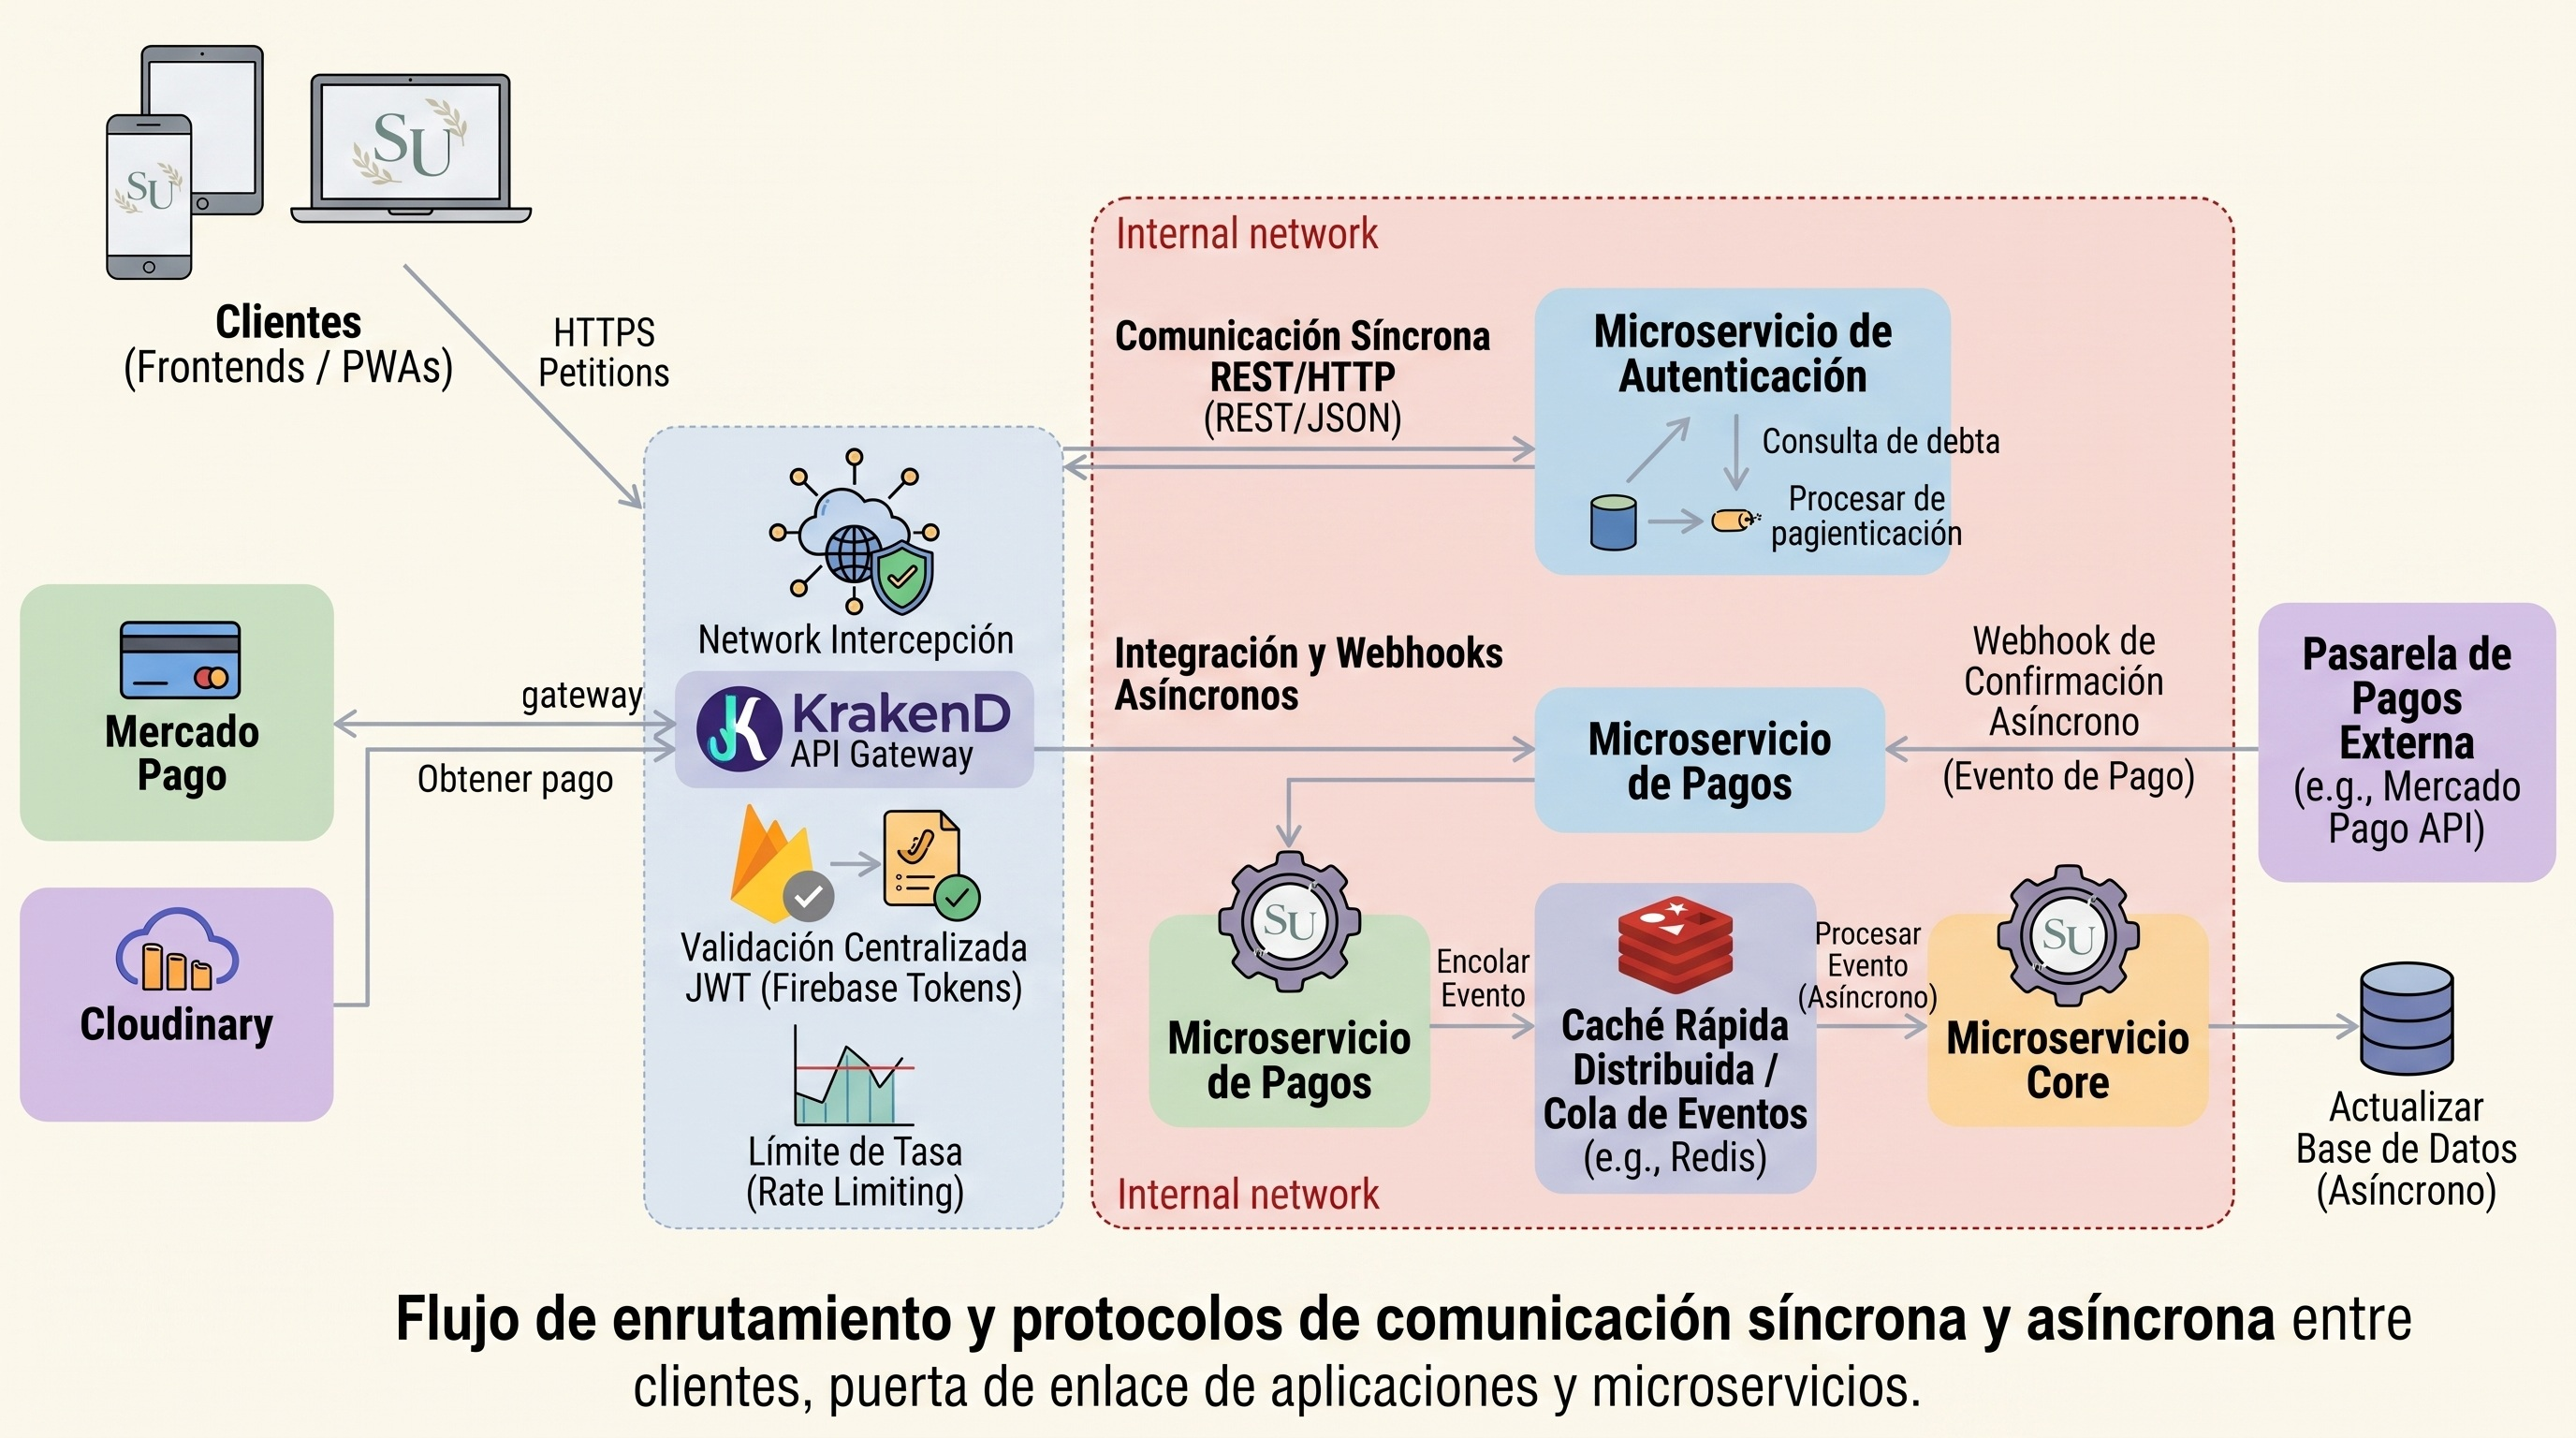
\includegraphics[width=\textwidth]{img/arquitectura/diagrama.jpg}}
    \caption{Flujo de enrutamiento y protocolos de comunicación síncrona y asíncrona entre clientes, puerta de enlace de aplicaciones y microservicios.}
    \label{fig:comunicacion_servicios}
\end{figure}

\subsubsection{Catálogo y responsabilidades de los microservicios}

El núcleo de la solución se desglosa en un catálogo de microservicios aislados, desplegados en contenedores independientes que manejan sus propias bases de datos transaccionales de Neon (PostgreSQL serverless en la nube) u otros esquemas adaptados:

\begin{enumerate}
    \item \textbf{Puerta de enlace de API (API Gateway - gateway)}: Desarrollado sobre el motor declarativo de \textit{KrakenD}. Al ser el punto de entrada unificado y público del ecosistema, este componente está programado internamente en Go (\textit{Golang}), lo que garantiza una concurrencia masiva capaz de procesar miles de peticiones por segundo con un consumo mínimo de memoria. Su arquitectura es estrictamente sin estado (\textit{stateless}) y se encarga de interceptar todas las peticiones entrantes desde los clientes de \textit{frontend}, validar de manera centralizada la firma y vigencia de los tokens \textit{JWT} emitidos por Firebase, aplicar políticas estrictas de limitación de tasa (\textit{rate limiting}) para evitar abusos o ataques de denegación de servicio, y enrutar de forma segura el tráfico limpio hacia los microservicios correspondientes de la red interna.
    \item \textbf{Microservicio central (Core - microservicio-club)}: Desarrollado en Python con FastAPI. Es el encargado de procesar la lógica de negocio central del club, abarcando la creación de categorías de socios, el manejo del padrón societario, el control de las inscripciones a disciplinas deportivas y la orquestación del calendario de reserva de instalaciones.
    \item \textbf{Microservicio de pagos (microservicio-pagos)}: Construido en Python con FastAPI. Gestiona las integraciones directas con las pasarelas transaccionales de Mercado Pago y los correos automatizados mediante Resend. Es el encargado de recibir notificaciones de cobro y conciliar el flujo contable.
    \newpage
    \item \textbf{Microservicio de acceso inteligente (microservicio-acceso)}: Desarrollado en Python utilizando el \textit{framework} FastAPI. La persistencia transaccional y el control de las migraciones se gestionan mediante el mapeador objeto-relacional (\textit{ORM}) SQLAlchemy y Alembic respectivamente, permitiendo un modelado de base de datos robusto y un versionado de esquemas incremental para las tablas de accesos y secretos. El aseguramiento de la calidad de la lógica de validación de contraseñas de un solo uso basadas en tiempo (\textit{TOTP}) se realiza de forma continua utilizando el entorno de pruebas Pytest mediante accesorios (\textit{fixtures}) modulares. Por último, la paridad absoluta entre entornos se garantiza mediante la contenerización del servicio con Docker y Docker Compose.
    \item \textbf{Microservicio de autenticación (microservicio-autenticacion)}: Desarrollado en Python. Administra el ciclo de vida de los accesos y roles (socios, empleados, administradores, directores). Delega la administración física de contraseñas de manera segura en Firebase Authentication, encapsulando y emitiendo vales web seguros para la autorización perimetral del sistema.
    \item \textbf{Microservicio conversacional (microservicio-bot-conversacional)}: Desarrollado en Python utilizando la biblioteca de llamadas asíncronas de la API de Telegram. Se ejecuta mediante un proceso continuo de consulta activa (\textit{polling}) que captura las interacciones conversacionales de los usuarios, normaliza los textos libres y se conecta internamente con la API de core para procesar consultas de disciplinas, reservas o links de pago rápidos sin fricciones operativas.
    \item \textbf{Microservicio de analíticas (microservicio-analiticas)}: Procesa los tableros analíticos y los reportes consolidados para la dirigencia del club. Integra un almacenamiento rápido en caché mediante Redis para optimizar la latencia en las consultas financieras masivas agregadas.
    \item \textbf{Servicio de observabilidad (Healthchecker)}: Nodo sensor independiente y desacoplado del API Gateway, que vigila continuamente la disponibilidad física y lógica de todos los microservicios desplegados. Si se detecta un fallo, el panel de monitoreo expone visualmente el nodo degradado para facilitar la resiliencia proactiva del sistema de marca blanca.
\end{enumerate}

Cabe destacar que el desglose de componentes presentado en este catálogo constituye únicamente una síntesis conceptual a alto nivel de implementaciones de \textit{software} e infraestructura sumamente extensas y complejas. Con el propósito de asegurar la mantenibilidad a largo plazo, facilitar la incorporación de nuevos ingenieros al equipo y garantizar un traspaso tecnológico ordenado, cada repositorio de código fuente del ecosistema cuenta con su propia página de documentación técnica independiente desarrollada con la herramienta de código abierto \textit{Just the Docs}. En estos sitios documentales dedicados se expande detalladamente el listado completo de sus puntos de acceso (\textit{endpoints}), la justificación minuciosa de las elecciones tecnológicas adoptadas, las métricas clave de su implementación y los diagramas específicos de su arquitectura interna.

\subsection{Atributos de calidad y resiliencia arquitectónica}

La arquitectura y el diseño de \textbf{SocioUnido} fueron concebidos bajo lineamientos rigurosos de ingeniería de software, priorizando un conjunto de atributos de calidad que responden de manera directa a las necesidades críticas del ecosistema deportivo. A continuación, se detallan los pilares fundamentales que guían el desarrollo de la plataforma:

\subsection{Seguridad}

Representa uno de los pilares centrales del sistema. Dado que la plataforma gestiona información altamente sensible (datos personales, registros financieros y credenciales de acceso), se aplican estrictas medidas de protección para garantizar la confidencialidad, la privacidad y la integridad absoluta de los datos, resguardando tanto a los clubes como a su masa societaria frente a posibles vulnerabilidades.

\newpage

\subsection{Escalabilidad}

La arquitectura de la plataforma tiene el propósito fundamental de priorizar la adaptabilidad ante variaciones de carga. Al adoptar un diseño modular basado en microservicios, el sistema permite escalar cada componente de forma independiente según la demanda específica de recursos. Esta separación de responsabilidades facilita alcanzar cotas de rendimiento sumamente altas sin comprometer la estabilidad global de la aplicación.

\subsection{Disponibilidad y resiliencia}

Debido al flujo continuo de personas en las instalaciones del club y a la existencia de momentos operativos críticos (como los días de partido o eventos de asistencia masiva), el sistema exige un tiempo de actividad (\textit{uptime}) máximo. Se diseñaron estrategias de mitigación para cortar posibles vectores de ataque y aislar problemas técnicos, asegurando que un fallo aislado no derive en una interrupción total del servicio.

\subsection{Rendimiento y eficiencia}

Si bien la seguridad y la disponibilidad son los núcleos de la arquitectura, el rendimiento es un factor clave para garantizar una adopción exitosa. Se optimizó el consumo de recursos y los tiempos de respuesta para ofrecer una interacción fluida y ágil, logrando que el uso diario de la aplicación resulte una experiencia agradable y no represente un obstáculo burocrático o tecnológico para el usuario.

\subsection{Usabilidad y accesibilidad}

En estrecha relación con el rendimiento, la interfaz y los flujos de trabajo fueron diseñados para reducir al mínimo la fricción operativa. Para alcanzar este estándar, se llevaron a cabo exhaustivas reuniones de validación de producto, se realizaron encuestas y se procesó un volumen significativo de \textit{feedback} provisto por los propios usuarios. Esto permitió pulir el sistema para que sea intuitivo y accesible frente a una demografía con distintos niveles de alfabetización digital.

\subsection{Interoperabilidad}

La capacidad del sistema para integrarse con actores y sistemas externos se centró estratégicamente en dos frentes de expansión futura. En primer lugar, la aplicación está estructurada para facilitar la interacción directa con modelos de inteligencia artificial y agentes autónomos; ante el actual superciclo de innovación tecnológica, resulta indispensable contar con interfaces preparadas por si esta modalidad se consolida como el estándar masivo de interacción. En segundo lugar, el diseño contempla la futura integración a nivel de \textit{hardware} (como la conexión con molinetes y controles de acceso físicos) para agilizar y blindar de forma definitiva el ingreso a los recintos deportivos.

\newpage

\subsection{Impacto de las Prácticas Profesionales Supervisadas (PPS)}La consolidación de \textbf{SocioUnido} como un producto de alto estándar técnico y comercial es el resultado directo de la aplicación de los conocimientos adquiridos durante las Prácticas Profesionales Supervisadas (PPS) correspondientes a la asignatura Emprendimientos Basados en Tecnología 2 y su materia precursora. Esta base metodológica, forjada durante el trayecto formativo en la Facultad de Ingeniería de la Universidad de Buenos Aires (FIUBA), fue determinante para escalar el proyecto más allá de un simple prototipo, transformándolo en un ecosistema integral preparado para competir en el mercado real de la gestión deportiva.  El éxito en la ejecución de este Trabajo Profesional se apoya en los siguientes pilares derivados de dichas prácticas:\begin{itemize}
    \item \textbf{Visión comercial y validación empírica:} Desde su concepción, el sistema fue tratado como un producto real, respaldado por la creación de una identidad de marca, una página publicitaria de captación y un canal oficial de medios. Además, su enfoque funcional se validó de forma empírica y constante mediante iteraciones, reuniones con trabajadores de clubes reales y encuestas de usabilidad orientadas a los usuarios finales.
    \item \textbf{Gestión ágil y control de calidad:} La organización del equipo se estructuró de manera profesional bajo el marco \textit{Scrum} y la metodología Kanban. Esto permitió gestionar el desarrollo continuo del producto a lo largo de 13 \textit{sprints}, priorizar historias de usuario y monitorear proactivamente la resolución de errores (\textit{bugs}), esfuerzo que quedó documentado en el registro de horas de las PPS.
    \item \textbf{Análisis de viabilidad y proyecciones de inversión:} Aplicando las herramientas analíticas de formulación de proyectos, se elaboró un estudio económico-financiero para evaluar las inversiones iniciales requeridas, los costos operativos de la infraestructura en la nube y la escalabilidad del modelo de negocio. Este análisis permitió estructurar la sustentabilidad del ecosistema bajo un esquema comercial de \textit{software} como servicio (B2B SaaS), garantizando su viabilidad en el mercado real de la gestión deportiva.
    \item \textbf{Estrategia legal y protección de la propiedad intelectual:} Para resguardar el valor tecnológico del producto (arquitecturas distribuidas, algoritmos de inteligencia artificial y validación criptográfica), se definió un marco legal robusto adoptando la licencia \textit{PolyForm Noncommercial License 1.0.0}. Esta decisión estratégica protege los derechos de explotación comercial exclusiva del equipo desarrollador frente a terceros, garantizando de manera simultánea que el código fuente permanezca abierto, auditable y accesible para fomentar la revisión entre pares dentro del ámbito académico de la universidad.
\end{itemize}
